\chapter{DESAIN DAN IMPLEMENTASI SISTEM}
\label{sec:chap3}

\section{Deskripsi Sistem}

Bab ini menjelaskan perancangan dan implementasi sistem robot inspeksi berbasis agen \textit{Multimodal Large Language Model} (MLLM) yang dibangun di atas platform Jueying Lite3. Sistem ini dirancang agar operator dapat mengendalikan robot melalui instruksi bahasa alami, di mana agen AI akan secara otonom merencanakan dan mengeksekusi misi inspeksi secara bertahap dengan verifikasi operator di setiap langkahnya.

\subsection{Gambaran Umum Sistem}
Gambar \ref{fig:high_level_diagram} menunjukkan diagram umum dari keseluruhan sistem. Secara garis besar, sistem yang diusulkan dirancang untuk menjembatani kesenjangan komunikasi antara operator manusia dan robot \textit{quadruped} melalui antarmuka bahasa alami. Berbeda dengan metode teleoperasi konvensional yang mengandalkan kendali manual penuh, sistem ini menempatkan \textit{Multimodal Large Language Model} (MLLM) sebagai unit pemroses logika pusat yang mengorkestrasi alur informasi dari instruksi pengguna hingga eksekusi fisik robot. Skema interaksi ini mengubah cara kerja sistem pengendalian robot dari yang sebelumnya bersifat teknis dan kaku menjadi lebih intuitif dan semantik.

\begin{figure}[H]
    \centering
    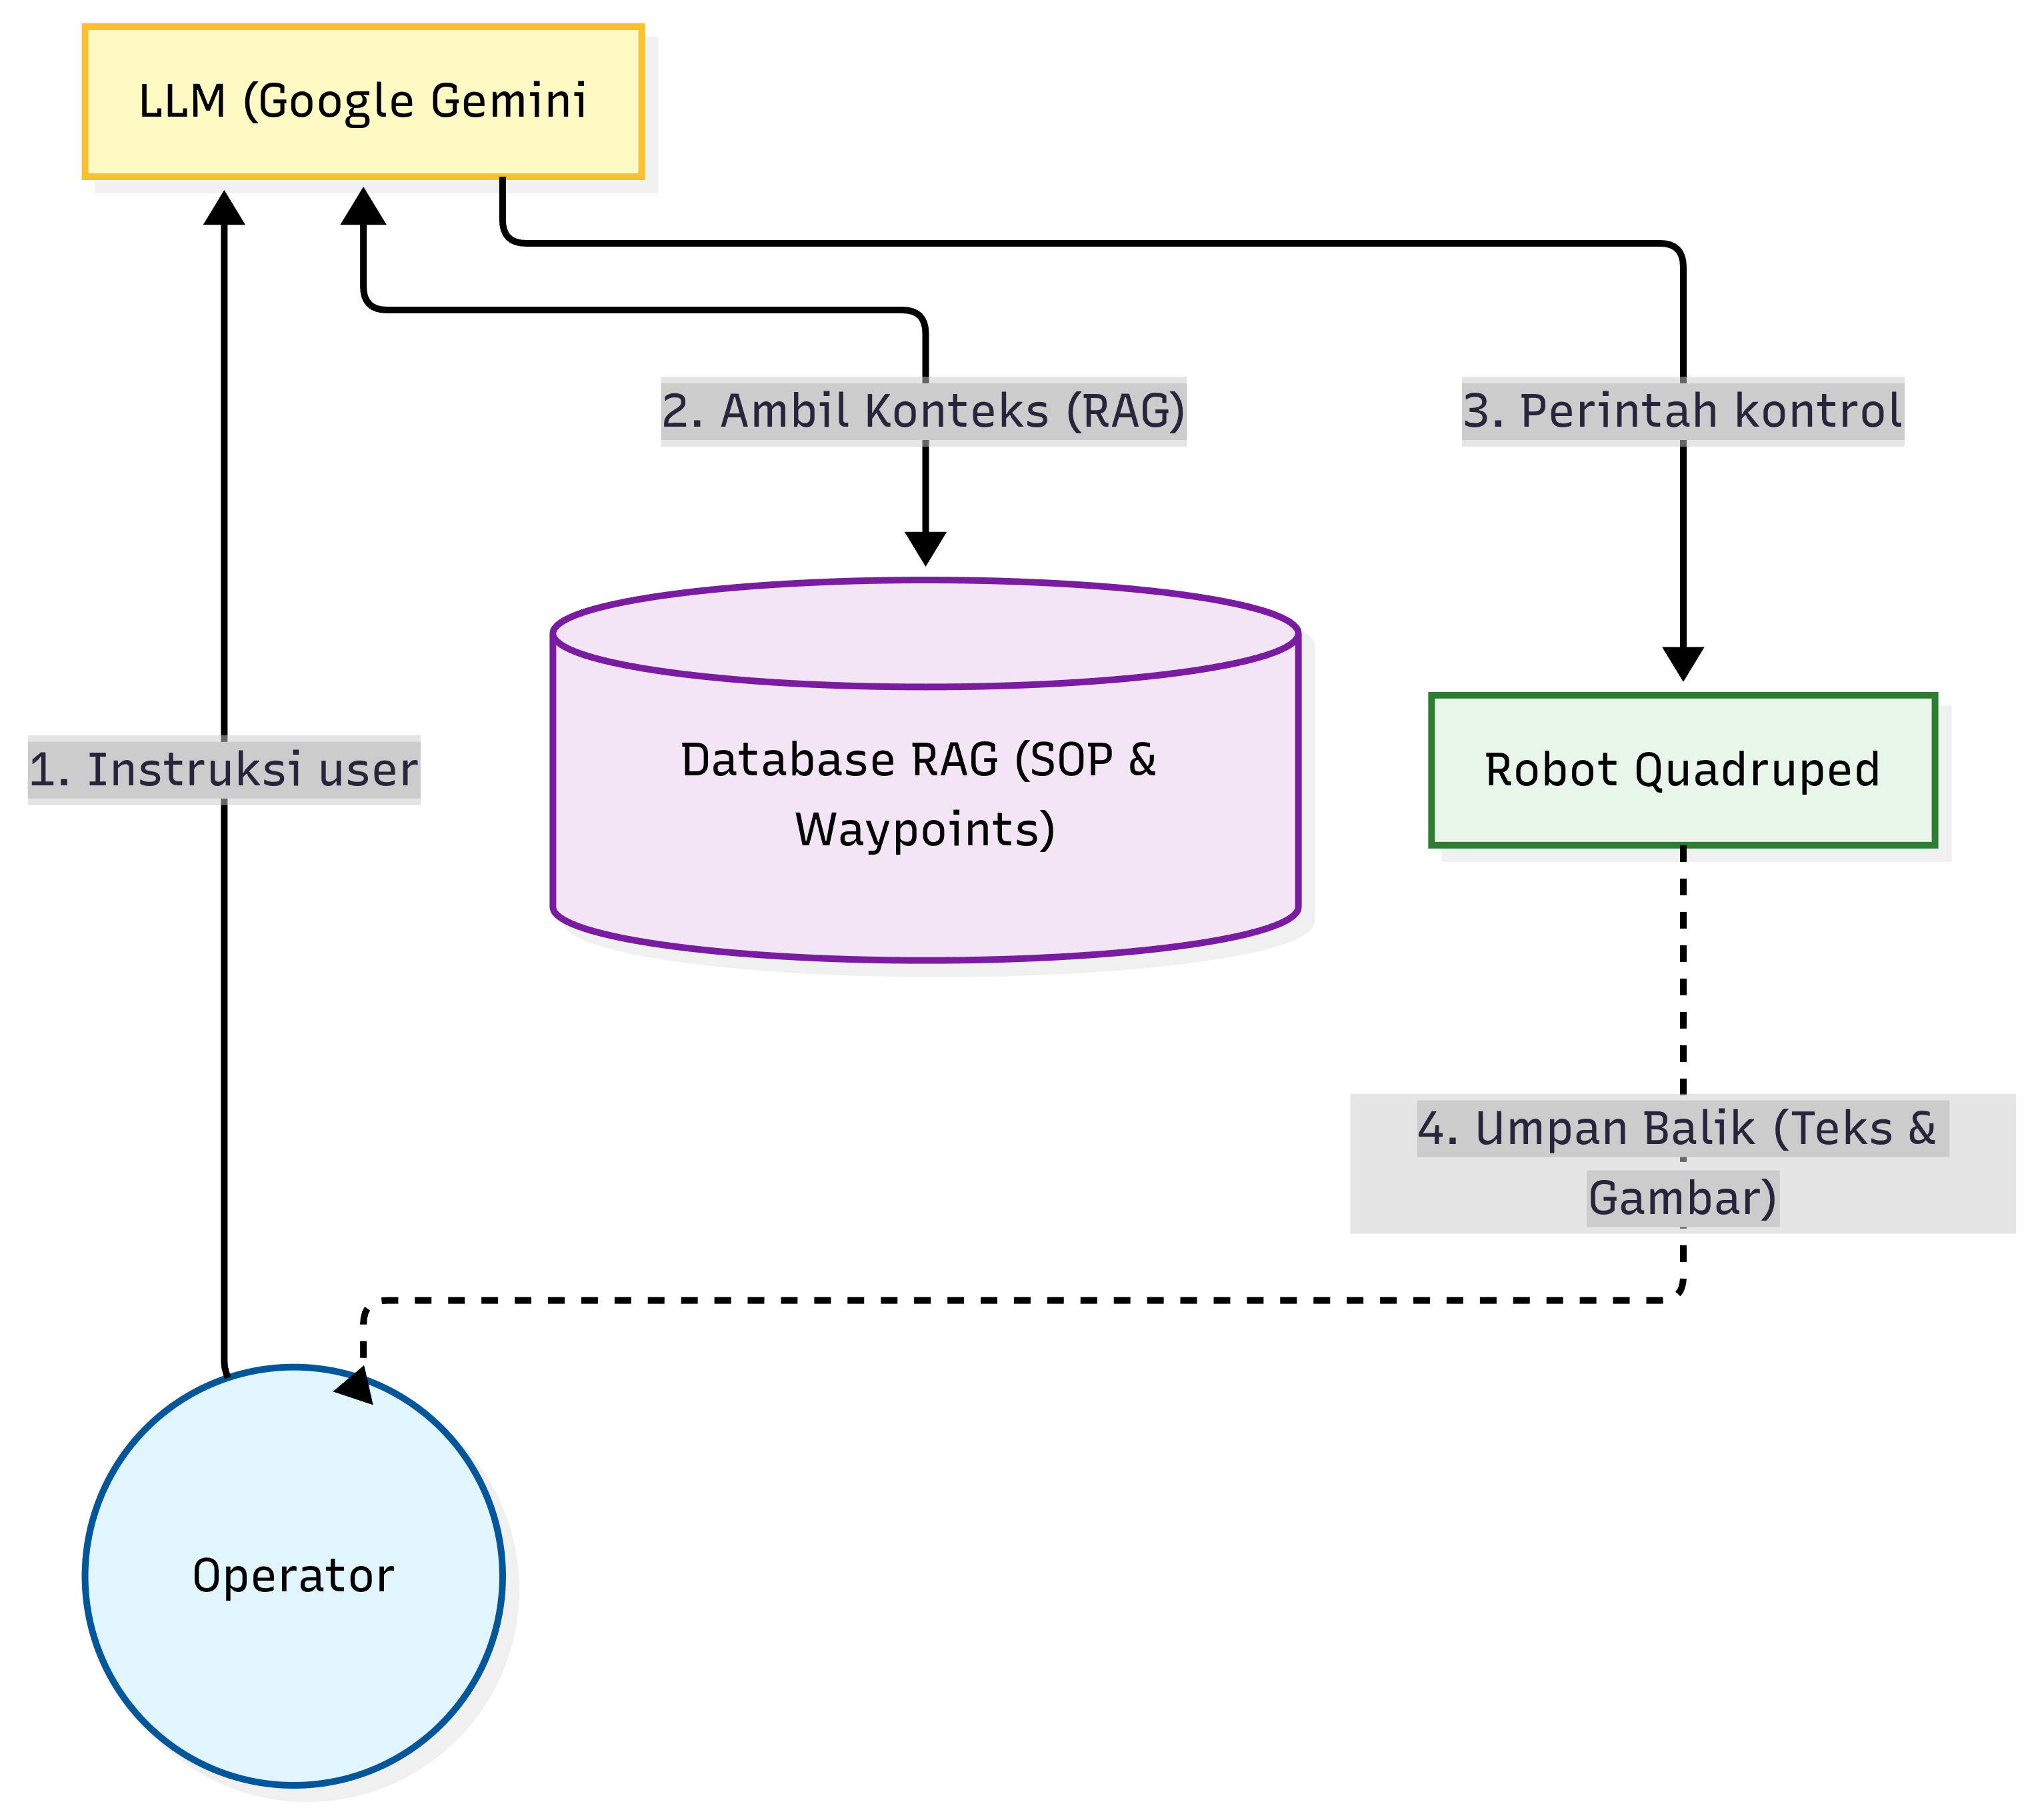
\includegraphics[width=0.5\textwidth]{Init/gambar/umum.png} 
    \caption{Diagram Umum Sistem}
    \label{fig:high_level_diagram}
\footnotesize \textbf{Sumber:} Dokumentasi Penulis
\end{figure}

Mekanisme kerja sistem diawali dengan pemberian instruksi oleh operator menggunakan bahasa alami berupa nama objek target inspeksi. Perintah abstrak ini kemudian diproses oleh MLLM, namun tidak langsung diterjemahkan secara harfiah. MLLM secara aktif melakukan pencarian konteks (\textit{Context Retrieval} dengan pendekatan \textit{Agentic RAG}) ke basis data eksternal melalui pemanggilan \textit{tools} untuk mengambil informasi pendukung yang relevan, seperti peta semantik, titik koordinat \textit{waypoints}, serta dokumen \textit{Standard Operating Procedure} (SOP) yang berkaitan dengan objek inspeksi. Langkah ini krusial untuk memastikan bahwa keputusan yang diambil oleh MLLM didasarkan pada data spasial dan prosedural yang akurat, bukan sekadar halusinasi model bahasa.

Setelah pemahaman kontekstual terbentuk, MLLM tidak secara langsung memerintah robot, melainkan menyusun rencana inspeksi dan mengeksekusinya melalui serangkaian pemanggilan \textit{tools}. Pemanggilan \textit{tools} inilah yang kemudian meneruskan perintah navigasi dan kontrol ke robot \textit{quadruped} untuk dieksekusi, menggerakkan aktuator fisik menuju lokasi target secara otonom. Sistem ini menerapkan mekanisme eksekusi secara bertahap. Setelah menyelesaikan suatu aksi navigasi atau pengambilan data, sistem akan mengirimkan laporan status beserta bukti visual kembali kepada operator. Mekanisme ini memberikan kesempatan bagi operator untuk memvalidasi hasil tindakan robot sebelum sistem diizinkan mengeksekusi \textit{tool} tahap berikutnya, sehingga menjamin keamanan dan adaptabilitas operasi inspeksi di lingkungan yang dinamis.

\subsection{Arsitektur Sistem}
Arsitektur sistem dalam penelitian ini menggunakan pendekatan terdistribusi yang mengintegrasikan kemampuan penalaran tingkat tinggi dari \textit{Multimodal Large Language Model} (MLLM) dengan sistem kendali robotik. Kompo\-nen-kompo\-nen sistem dirancang secara modular dan saling terhubung melalui jaringan TCP/IP lokal maupun internet. Gambaran menyeluruh mengenai arsitektur sistem dan topologi data disajikan pada Gambar \ref{fig:arsitektur_sistem}.

\begin{figure}[H]
    % Pastikan diagram mermaid baru sudah di-export jadi gambar
    \centering
    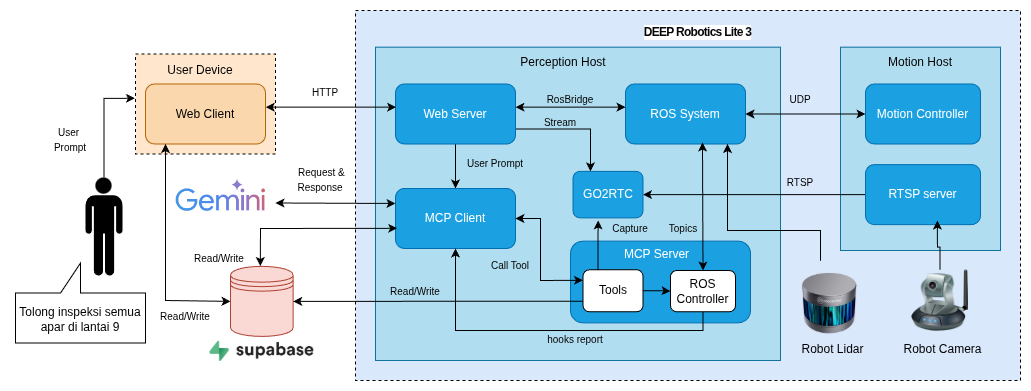
\includegraphics[width=1.0\textwidth]{Init/gambar/arsitektur_new.png}
    \caption{Diagram Arsitektur Sistem}
    \label{fig:arsitektur_sistem}
    \footnotesize \textbf{Sumber:} Dokumentasi Penulis
\end{figure}


\subsubsection{Google Gemini API}
Google Gemini API merupakan komponen yang berperan sebagai otak pemroses utama untuk sistem inspeksi. Pemilihan model Gemini didasarkan pada keunggulannya yang memiliki rasio nilai performa berbanding harga paling baik di antara model \textit{multimodal} lainnya di pasaran, sembari tetap mempertahankan kemampuannya dalam memproses analisis visual secara \textit{zero-shot} tanpa memerlukan pelatihan ulang pada data kustom. Gemini berfungsi untuk memahami perintah bahasa alami dari operator yang dikirim melalui \textit{Web Client}. Perintah tersebut dianalisis untuk membuat rencana inspeksi. Gemini menggunakan fitur \textit{function calling} untuk mengakses berbagai \textit{tools} yang ada pada MCP Server. Dengan fitur ini, Gemini bisa memutuskan kapan harus menggerakkan robot, kapan harus mengambil foto, atau kapan harus mencari dokumen SOP di \textit{database}. Gemini API juga berperan dalam proses analisis visual pada saat inspeksi berlangsung. Ketika kamera robot menangkap \textit{image} sebuah objek, \textit{image} tersebut dikirim ke Gemini API bersamaan dengan instruksi dari dokumen SOP. Gemini akan membandingkan kondisi visual objek pada foto dengan standar yang tertulis di SOP. Detail implementasi dari komponen ini dijelaskan pada Subbab 3.2.2.6.

\subsubsection{Supabase}
Supabase dalam sistem ini diimplementasikan sebagai platform pusat penyimpanan data yang digunakan oleh \textit{Web Client}, \textit{MCP Client}, dan \textit{MCP Server}. Penggunaan platform Supabase pada arsitektur ini didasarkan pada kebutuhan sistem akan penyatuan fungsional antara basis data relasional dan penyimpanan berkas objek di dalam satu ekosistem yang tersinkronisasi. Fungsi pertama dari Supabase adalah sebagai \textit{database} relasional. Di dalam \textit{database} ini, sistem menyimpan daftar lokasi dan koordinat target. Selain itu, \textit{database} juga digunakan untuk menyimpan log \textit{Session History} yang berisi riwayat percakapan antara operator dan Gemini agar konteks memori misi sebelumnya tetap terjaga. Fungsi kedua adalah sebagai \textit{Storage} untuk menyimpan dokumen dan \textit{image}. Komponen penyimpanan ini digunakan secara spesifik untuk menyimpan fail dokumen SOP, serta setiap foto hasil tangkapan kamera robot saat proses inspeksi di lapangan berlangsung. Detail implementasi dari komponen ini dijelaskan pada Subbab 3.2.5.

\subsubsection{\textit{Web App}}
\textit{Web App} merupakan antarmuka utama yang digunakan oleh operator untuk mengendalikan dan memantau robot. \textit{Web App} ini dijalankan di dalam PC internal robot dan difungsikan secara spesifik untuk memfasilitasi peran pengawasan manusia (\textit{Human-in-the-Loop}). Komponen ini bertindak sebagai media komunikasi antara operator dan \textit{AI Agent} melalui panel \textit{chat}. Selain itu, \textit{Web App} juga menyediakan fitur manajemen data untuk mengatur lokasi \textit{waypoint} target dan mengelola dokumen panduan inspeksi. Fungsi lainnya adalah sebagai pusat pemantauan \textit{real-time}, di mana komponen ini mengeksekusi pemuatan aliran video secara langsung dari kamera robot menggunakan protokol WebRTC serta menampilkan data telemetri robot melalui koneksi \textit{Rosbridge WebSocket}. Detail implementasi dari komponen ini dijelaskan pada Subbab 3.2.1.

\subsubsection{MCP \textit{Client}}
MCP \textit{Client} dirancang sebagai perantara komunikasi (\textit{middleware}) antara antarmuka web, Gemini API, dan MCP Server dalam menjalankan mekanisme \textit{Agentic Loop}. Komponen MCP \textit{Client} ini mengeksekusi tiga logika krusial. Pertama, komponen ini mengelola \textit{System Prompt} untuk menginjeksikan konfigurasi kepribadian serta batasan operasional yang harus dipatuhi oleh Gemini sebelum pesan dikirim. Kedua, ketika Gemini menghasilkan balasan berupa pemanggilan alat bantu (\textit{function calling}), komponen ini menerjemahkan pesan perintah tersebut menjadi instruksi berformat HTTP dan meneruskannya ke \textit{tools} yang sesuai pada MCP Server. Ketiga, setelah memperoleh respons balasan dari robot, komponen ini akan mengirimkan kembali hasil tersebut kepada Gemini sekaligus menyinkronkan data interaksi riwayat percakapan ke dalam \textit{database} Supabase. Detail implementasi dari komponen ini dijelaskan pada Subbab 3.2.2.

\subsubsection{MCP \textit{Server}}
MCP Server beroperasi sebagai lapisan abstraksi dieksekusi di dalam robot. Komponen ini bertugas mengekspos seluruh fungsionalitas sistem operasi robot (ROS) menjadi kumpulan \textit{tools} sederhana yang siap dipanggil oleh agen AI dari luar. Komponen server ini, bertugas mendengarkan perintah pemanggilan \textit{tools} dari agen AI melalui MCP Client, lalu mengeksekusinya. \textit{Tools} ini mencakup pengiriman instruksi bergerak menggunakan fungsionalitas ROS, penangkapan \textit{image} dari kamera robot, pencarian koordinat \textit{waypoint} dan dokumen SOP dari basis data, hingga pelaksanaan komputasi analisis \textit{image}. Selain itu, komponen MCP Server juga mengeksekusi mekanisme \textit{webhook} untuk mengirimkan status ke MCP \textit{Client} setelah aksi pergerakan robot selesai. Detail implementasi dari komponen ini dijelaskan pada Subbab 3.2.3.

\subsubsection{Sistem ROS}
ROS berperan sebagai sistem yang mengelola seluruh komunikasi dan tugas navigasi pada robot. Di dalam komponen ROS ini, terdapat \textit{node} spesifik yang beroperasi, di antaranya adalah \textit{Navigation Stack} yang memproses data mentah lidar untuk menghasilkan peta lingkungan serta mengeksekusi perencanaan jalur (\textit{path planning}) selama misi berlangsung. Seluruh koordinasi pergerakan fisik dikelola melalui koneksi UDP menuju \textit{Motion Host}. Untuk menjembatani komunikasi dengan antarmuka luar, \textit{RosBridge Server} digunakan untuk mengeksekusi pembukaan protokol \textit{WebSocket} yang memungkinkan \textit{Web App} mengakses data telemetri robot. Integrasi antara ekosistem ROS dengan MCP Server dilakukan melalui mekanisme \textit{topics} yang memungkinkan \textit{tools} pada server mengakses fungsionalitas pergerakan robot. Detail implementasi dari komponen ini dijelaskan pada Subbab 3.2.4.

\subsubsection{\textit{Motion Controller}}
\textit{Motion Controller} merupakan unit kendali fisik tingkat terendah (\textit{low-level}) bawaan yang tertanam dan berinteraksi langsung dengan perangkat keras robot Jueying Lite3. Komponen ini ditempatkan di posisi paling ujung dalam rantai perintah pergerakan. Di dalam subsistem ini, dieksekusi proses komputasi yang memegang kendali atas keseimbangan dinamis mekanik dan rotasi sendi-sendi aktuator kaki (\textit{gait planning}). Komponen ini bertugas menerima perintah vektor abstraksi kecepatan (\textit{velocity command}) dari ekosistem ROS, lalu mengeksekusi penerjemahannya menjadi sinyal daya putaran torsi motor yang secara aktual menggerakkan fisik robot. Detail implementasi dari komponen ini dijelaskan pada Subbab 3.2.4.4.

\subsubsection{GO2RTC}
 Komponen GO2RTC digunakan untuk mengelola distribusi aliran data visual dari kamera robot menuju berbagai modul dalam sistem. Komponen ini menerima aliran data bervolume tinggi melalui protokol RTSP dari \textit{RTSP server} yang terhubung langsung dengan perangkat keras kamera pada \textit{Motion Host}. GO2RTC kemudian mengeksekusi konversi aliran protokol transmisi tersebut menjadi format WebRTC agar dapat diakses dengan latensi sekecil mungkin oleh modul \textit{Web App} dan MCP Server. Detail implementasi dari komponen ini dijelaskan pada Subbab 3.2.1.1 dan Subbab 3.2.3.7.

\subsubsection{RTSP \textit{Server}}
RTSP \textit{server} beroperasi di dalam modul \textit{Motion Host} sebagai penyedia akses data visual mentah yang bersumber langsung dari kamera robot. Di dalam siklus kerjanya, komponen ini memiliki tanggung jawab untuk mengeksekusi pengambilan data \textit{image}, mengelola aliran data video tersebut, dan menyediakannya dalam format transmisi standar melalui protokol \textit{Real-Time Streaming Protocol} agar dapat dikonsumsi oleh komponen distribusi lanjutan seperti GO2RTC. Detail implementasi dari komponen ini dijelaskan pada Subbab 3.2.1.1 dan Subbab 3.2.3.7.

\subsection{Alur Sistem}

Alur kerja dari sistem inspeksi visual otonom ini dibagi menjadi tiga fase utama, yaitu fase perencanaan, fase eksekusi dan analisis, serta fase pelaporan hasil. Interaksi data dan pesan antarkomponen untuk menyelesaikan sebuah misi divisualisasikan melalui diagram sekuensial pada Gambar \ref{fig:sequence_diagram}. 

\begin{figure}[H]
    \centering
    \includegraphics[width=0.8\textwidth]{Init/gambar/alur_baru.png}
    \caption{Diagram Sekuensial Alur Interaksi Sistem}
    \label{fig:sequence_diagram}
\footnotesize \textbf{Sumber:} Dokumentasi Penulis
\end{figure}

Diagram sekuensial pada Gambar \ref{fig:sequence_diagram} merepresentasikan lima aktor utama (ditunjukkan oleh kotak di bagian atas) yang berpartisipasi dalam siklus sistem, yaitu: Operator manusia, Agen AI (bertindak sebagai MCP \textit{Client}), MCP \textit{Server}, Supabase (sebagai pusat basis data), dan fisik robot \textit{quadruped} (menjalankan ROS dan kamera). Garis lurus tebal (\textit{solid line}) yang mengarah dari satu aktor ke aktor lain menggambarkan pengiriman perintah atau permintaan (\textit{request}), sedangkan garis putus-putus (\textit{dashed line}) menggambarkan pengembalian data atau respons (\textit{callback/return}). Kotak vertikal panjang yang berada di bawah setiap aktor merepresentasikan waktu aktif (\textit{lifeline}) di mana komponen tersebut sedang memproses suatu tugas. Seluruh komponen ini bekerja secara sinkron dan saling melengkapi melalui tiga fase utama berikut.

\subsubsection{Fase Perencanaan}

Fase perencanaan berfokus pada penerimaan instruksi abstrak dari manusia dan penyusunan rencana kerja terstruktur oleh sistem sebelum robot melakukan pergerakan fisik. Seperti yang diilustrasikan pada sepertiga awal diagram, proses interaksi pesan pada fase ini diuraikan sebagai berikut:

\begin{enumerate}
    \item \textbf{\textit{User Prompt}:} Operator memasukkan perintah bahasa alami melalui panel obrolan (\textit{chat}) pada antarmuka web, yang langsung diteruskan kepada agen AI (gabungan MCP \textit{Client} dan Gemini).
    \item \textbf{\textit{Execute Tool} Pencarian:} Merespons instruksi tersebut, agen AI mengirimkan perintah ke MCP Server untuk mengeksekusi \textit{tool} pencarian data koordinat objek (\textit{waypoint}) dan dokumen SOP.
    \item \textbf{\textit{Query Data}:} MCP Server meneruskan perintah tersebut dengan melakukan kueri ke basis data Supabase.
    \item \textbf{\textit{Return Coordinates \& SOP Content}:} Supabase merespons dengan mengembalikan data titik koordinat spasial beserta isi panduan inspeksi secara terstruktur.
    \item \textbf{\textit{Tool Result}:} MCP Server meneruskan data hasil pencarian tersebut kembali kepada agen AI sebagai konteks misi.
    \item \textbf{\textit{Plan Result}:} Agen AI memproses seluruh data konteks, menghasilkan draf rencana inspeksi secara utuh, dan menampilkannya kembali ke layar antarmuka Operator untuk ditinjau.
    \item \textbf{\textit{User Confirmation}:} Di titik pengawasan ini, Operator memberikan persetujuan eksplisit untuk mengesahkan rencana kerja sebelum robot diberi izin untuk mulai bergerak.
\end{enumerate}

\subsubsection{Fase Eksekusi dan Analisis}

Fase kedua merupakan tahap di mana sistem mulai menggerakkan perangkat keras robot dan melakukan pemrosesan visual berdasarkan rencana yang telah disetujui. Langkah-langkah interaksi pada fase ini adalah sebagai berikut:

\begin{enumerate}
    \setcounter{enumi}{7}
    \item \textbf{\textit{Execute Tool Navigation}:} Setelah konfirmasi dari operator, agen AI mengirimkan perintah ke MCP Server untuk mengeksekusi \textit{tool} navigasi pergerakan fisik.
    \item \textbf{\textit{Send ROS Messages}:} MCP Server menerjemahkan perintah abstrak tersebut dengan menembakkan pesan instruksi teknis ke dalam sistem ROS pada robot agar mulai bergerak secara otonom.
    \item \textbf{\textit{Status Running}:} Segera setelah perintah pergerakan terkirim, MCP Server membalas agen AI dengan status "running" agar siklus AI tidak membeku sembari menunggu perjalanan yang memakan waktu.
    \item \textbf{\textit{Status Arrived}:} Saat robot mencapai titik koordinat spasial yang dituju, sistem ROS mendeteksi keberhasilan navigasi dan mengirimkan status kedatangan ke MCP Server.
    \item \textbf{\textit{Webhook Report}:} MCP Server meneruskan status kedatangan tersebut dengan mekanisme \textit{webhook} kepada agen AI untuk memicu \textit{agent loop} kembali.
    \item \textbf{\textit{Execute Tool Capture}:} Agen AI langsung mengirimkan perintah lanjutan kepada MCP Server untuk mengeksekusi pengambilan \textit{image}.
    \item \textbf{\textit{Capture Image}:} MCP Server menjalankan perintah pengambilan \textit{image} ini dengan cara mengakses kamera melalui GO2RTC.
    \item \textbf{\textit{Image Result}:} GO2RTC pada robot merespons dengan mengembalikan biner \textit{image} secara utuh kembali kepada MCP Server.
    \item \textbf{\textit{Save Image}:} MCP Server mengirimkan \textit{image} tersebut ke basis data Supabase untuk diarsipkan ke dalam \textit{Storage}.
    \item \textbf{\textit{Image URL \& Analysis Result}:} Bersamaan dengan itu, MCP Server melampirkan tautan URL \textit{image} serta mengembalikan hasil analisis \textit{image} kembali kepada agen AI agar dapat difinalisasi.
\end{enumerate}

\subsubsection{Fase Pelaporan}

Fase pelaporan merupakan tahap penutup dari satu siklus inspeksi objek tunggal, di mana hasil kerja robot dilaporkan dan keputusan kelanjutan misi dikembalikan ke tangan manusia. Rincian percabangan pesannya adalah sebagai berikut:

\begin{enumerate}
    \setcounter{enumi}{17}
    \item \textbf{\textit{Show Analysis Result}:} Agen AI menyajikan narasi evaluasi akhir kondisi objek beserta bukti visual \textit{image} ke layar antarmuka obrolan agar dapat diperiksa langsung oleh Operator.
    \item \textbf{\textit{Interruption Prompt} (Skenario Intervensi):} Apabila Operator mendeteksi adanya kejanggalan pada foto visual yang ditayangkan, alur masuk ke percabangan di mana operator segera mengetikkan instruksi interupsi manual (misal: "Maju sedikit, foto lagi").
    \item \textbf{\textit{Execute Tools} (Skenario Intervensi):} Merespons interupsi, agen AI memberikan perintah eksekusi \textit{tool} sesuai instruksi interupsi operator melalui MCP Server.
    \item \textbf{\textit{User Confirmation} (Skenario Lanjut):} Sebaliknya pada jalur alternatif kedua, apabila Operator merasa puas dengan hasil analisis objek tersebut, ia memberikan izin persetujuan kepada AI untuk meneruskan sisa misinya.
    \item \textbf{\textit{Go To Next Waypoint} (Skenario Lanjut):} Setelah menerima izin kelanjutan, agen AI akan kembali mengeksekusi instruksi pergerakan ke titik lokasi target berikutnya. Seluruh siklus komunikasi dari nomor tujuh akan terus berulang hingga seluruh rangkaian rencana inspeksi terselesaikan.
\end{enumerate}

\subsection{Mekanisme (\textit{Human-in-the-Loop})}

Dalam arsitektur sistem ini, mekanisme \textit{Human-in-the-Loop} (HITL) diimplementasikan melalui panel obrolan (\textit{chat}) pada antarmuka web, di mana operator bertindak sebagai supervisor yang mengawasi dan menyetujui setiap keputusan agen AI. Agen AI diprogram melalui \textit{system prompt} untuk tidak mengeksekusi aksi robot atau memodifikasi rencana tanpa persetujuan eksplisit dari operator. Pendekatan ini tidak hanya meminimalisasi risiko kecelakaan atau kerusakan lingkungan akibat salah tafsir perintah, tetapi juga memberikan fleksibilitas tinggi bagi operator untuk menyesuaikan misi di lapangan.

Berdasarkan perancangan sistem, terdapat empat skenario utama kasus intervensi operator yang akan diuji untuk memvalidasi kapabilitas sistem:

\begin{enumerate}
    \item \textbf{Intervensi Perubahan Rencana Awal:} 
    Operator meminta perubahan rencana sesaat setelah agen AI menyusun \textit{inspection plan} namun sebelum robot bergerak. Contoh kasus: setelah sistem merencanakan inspeksi, operator mengintervensi dengan meminta agen untuk menambahkan instruksi agar robot mengambil posisi duduk setelah seluruh misi selesai.
    
    \item \textbf{Intervensi Penambahan Rencana di Tengah Misi:} 
    Operator memberikan instruksi baru saat robot sudah menjalankan sebagian misi. Contoh kasus: ketika robot baru saja selesai menginspeksi stop kontak dan bersiap ke tujuan berikutnya, operator meminta penambahan objek inspeksi baru (seperti tong sampah) ke dalam antrean rencana.
    
    \item \textbf{Intervensi Pembatalan Objek:} 
    Operator mengubah pikiran dengan membatalkan target inspeksi tertentu dan menggantinya dengan target lain. Contoh kasus: saat agen merencanakan inspeksi ke beberapa objek, operator menginstruksikan untuk membatalkan pemeriksaan pada satu stop kontak dan menukar beban tugasnya dengan menambah inspeksi pada satu tong sampah ekstra.
    
    \item \textbf{Intervensi Manuver:} 
    Operator memberikan intervensi untuk mengontrol pergerakan robot demi mendapatkan sudut pandang visual yang lebih baik ketika mendeteksi anomali. Contoh kasus: saat robot tiba di depan sebuah APAR yang kondisinya terlihat mencurigakan, operator menyuruh robot untuk "maju mendekat sedikit" sebelum memicu pengambilan \textit{image} ulang, guna memverifikasi kondisi objek dengan lebih jelas.
\end{enumerate}

Skenario-skenario intervensi ini merepresentasikan kondisi operasional dunia nyata yang dinamis, di mana sistem AI tidak boleh berjalan secara buta melainkan harus mampu beradaptasi dengan instruksi diskresi dari supervisor manusianya.

\subsection{Desain \textit{Web App}}

Desain antarmuka \textit{Web App} dirancang menggunakan pendekatan tata letak fungsional yang berfokus pada kemudahan \textit{monitoring} dan intervensi operator. Pembuatan rancangan awal (\textit{wireframe}) dari aplikasi web ini memuat beberapa halaman utama yang mendukung alur kerja inspeksi.

\subsubsection{Halaman Inspeksi}
\begin{figure}[H]
    \centering
    
\includegraphics[width=0.8\textwidth]{Init/gambar/wireframe/inspection_hub.png}
    \caption{Desain Antarmuka Halaman Inspeksi}
    \label{fig:desain_inspection_hub}
\footnotesize \textbf{Sumber:} Dokumentasi Penulis
\end{figure}
Halaman Inspeksi merupakan rancangan antarmuka utama di mana operator berinteraksi dengan sistem. Pada desain ini, tata letak dibagi menjadi panel percakapan di sisi kiri untuk berkomunikasi dengan agen AI, serta panel pemantauan di sisi kanan yang menayangkan aliran video secara langsung dari kamera robot dan representasi peta navigasi spasial. Selanjutnya, terdapat bar pada bagian atas untuk data telemetri robot.

\subsubsection{Halaman Manajemen Lokasi dan \textit{Waypoint}}
\begin{figure}[H]
    \centering
    
\includegraphics[width=0.8\textwidth]{Init/gambar/wireframe/spatial_explorer.png}
    \caption{Desain Antarmuka Halaman Manajemen Lokasi dan \textit{Waypoint}}
    \label{fig:desain_spatial_explorer}
\footnotesize \textbf{Sumber:} Dokumentasi Penulis
\end{figure}
Desain Halaman Manajemen Lokasi dan \textit{Waypoint} difokuskan untuk mempermudah operator dalam mengatur struktur data spasial. Antarmuka ini menampilkan hierarki lokasi dan tabel daftar koordinat target (\textit{waypoint}) yang memungkinkan operator untuk menambah, mengubah, atau menghapus titik tujuan inspeksi di dalam basis data.

\subsubsection{Halaman Manajemen SOP}
\begin{figure}[H]
    \centering
    
\includegraphics[width=0.8\textwidth]{Init/gambar/wireframe/sop.png}
    \caption{Desain Antarmuka Halaman Manajemen SOP}
    \label{fig:desain_sop_manager}
\footnotesize \textbf{Sumber:} Dokumentasi Penulis
\end{figure}
Rancangan Halaman Manajemen SOP bertujuan untuk memfasilitasi pengelolaan dokumen SOP inspeksi. Antarmuka ini menyediakan area khusus bagi pengguna untuk mengunggah berkas SOP secara langsung dengan mekanisme \textit{drag-and-drop} dan menampilkan daftar dokumen yang tersimpan dalam format \textit{grid} kartu untuk mempermudah pencarian.

\subsubsection{Halaman Riwayat Inspeksi}
\begin{figure}[H]
    \centering
    
\includegraphics[width=0.8\textwidth]{Init/gambar/wireframe/history.png}
    \caption{Desain Antarmuka Halaman Riwayat Inspeksi}
    \label{fig:desain_history_log}
\footnotesize \textbf{Sumber:} Dokumentasi Penulis
\end{figure}
Halaman Riwayat Inspeksi dirancang untuk menyajikan daftar seluruh sesi misi yang pernah dieksekusi. Desain antarmuka memuat tabel log sesi yang dilengkapi dengan fitur \textit{sliding panel}, sehingga operator dapat meninjau ulang isi percakapan dan analisis AI pada sesi terdahulu secara utuh.

\subsubsection{Halaman Galeri \textit{Image}}
\begin{figure}[H]
    \centering
    
\includegraphics[width=0.8\textwidth]{Init/gambar/wireframe/captured_gallery.png}
    \caption{Desain Antarmuka Halaman Galeri Tangkapan \textit{Image}}
    \label{fig:desain_image_gallery}
\footnotesize \textbf{Sumber:} Dokumentasi Penulis
\end{figure}
Desain Halaman Galeri \textit{Image} berfokus pada penyajian dokumentasi visual hasil inspeksi yang telah dilakukan sebelumnya. Tata letaknya menggunakan model \textit{grid} di mana setiap foto dari robot ditampilkan sebagai \textit{thumbnail} berserta informasi data penanda waktu pengambilan, dan dapat diperbesar untuk peninjauan lebih detail.

\subsubsection{Halaman Manajemen Objek}
\begin{figure}[H]
    \centering
    
\includegraphics[width=0.8\textwidth]{Init/gambar/wireframe/objects.png}
    \caption{Desain Antarmuka Halaman Manajemen Objek}
    \label{fig:desain_objects}
\footnotesize \textbf{Sumber:} Dokumentasi Penulis
\end{figure}
Halaman Manajemen Objek dirancang untuk mendefinisikan jenis objek yang akan diinspeksi. Antarmuka ini menampilkan tabel daftar nama objek beserta relasinya dengan pedoman SOP yang relevan dan kata kunci, guna membantu agen AI dalam mencari objek dan menyocokkan kondisi visual target dengan standar operasional.

\section{Implementasi Sistem}

Bagian ini membahas penerapan dari desain yang telah diuraikan sebelumnya. Implementasi sistem mencakup pengembangan antarmuka \textit{Web App} untuk operator, pembuatan modul MCP \textit{Client} sebagai jembatan komputasi agen AI, hingga integrasi pada MCP \textit{Server} yang secara fisik mengontrol pergerakan perangkat keras robot. Masing-masing realisasi modul perangkat lunak ini akan dijabarkan secara rinci pada subbab berikut.

\subsection{\textit{Web App}}

Antarmuka Web App dibangun menggunakan kerangka kerja Next.js dengan bahasa pemrograman TypeScript, dan dirancang sebagai \textit{Single Page Application} dengan sistem navigasi halaman internal yang dikelola melalui \textit{state manager}. Pengelolaan dan sinkronisasi data dari basis data Supabase maupun peladen FastAPI ditangani secara terpusat menggunakan pustaka TanStack React Query. Untuk kebutuhan pengontrolan robot, interaksi \textit{real-time} disalurkan melalui pustaka roslibjs yang terhubung langsung ke \textit{Rosbridge WebSocket} pada sistem robot. Aliran video dari kamera robot juga dirender secara langsung melalui protokol WebRTC yang bersumber dari komponen GO2RTC. Sementara itu, rancangan antarmuka dikonfigurasi menggunakan utilitas Tailwind CSS dan didukung oleh library GSAP untuk memberikan umpan balik animasi visual kepada operator.

\subsubsection{Halaman Inspeksi}
\begin{figure}[h!]
    \centering
    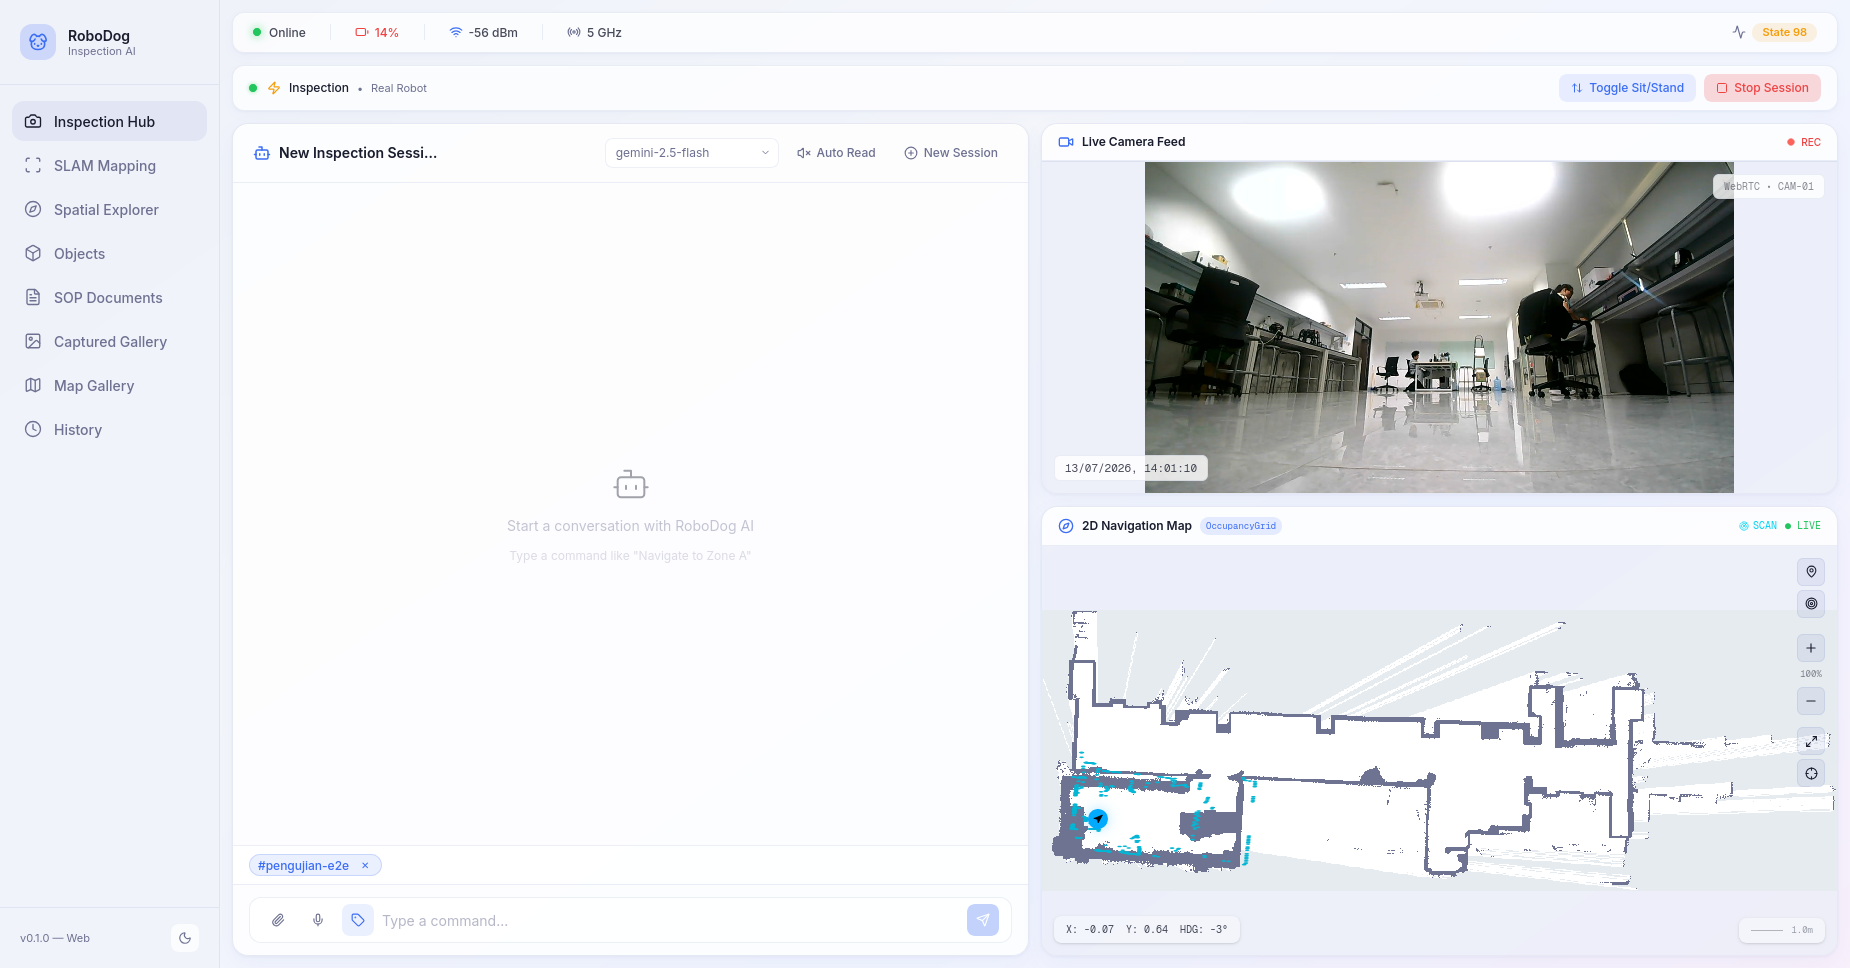
\includegraphics[width=0.8\textwidth]{Init/gambar/web_img/inspection_hub.png}
    \caption{Tampilan Halaman Inspeksi}
    \label{fig:inspection_hub}
\footnotesize \textbf{Sumber:} Dokumentasi Penulis
\end{figure}
Seperti yang ditampilkan pada Gambar \ref{fig:inspection_hub}, Halaman Inspeksi merupakan antarmuka utama bagi operator untuk mengendalikan misi robot secara interaktif. Sebelum memasuki antarmuka utama ini, operator disajikan dengan tombol untuk memulai peluncuran. Proses inisialisasi ini dipicu dengan mengeksekusi skrip inisialisasi navigasi robot quadruped berupa berkas bash melalui Next.js API route /api/shell di sisi server. Ketika sesi inisialisasi aktif dan terhubung, halaman akan memuat tata letak grid dinamis yang menggabungkan panel chat di sisi kiri serta panel video feed dan peta navigasi di sisi kanan.

Panel chat tersebut terhubung dengan Gemini API dan menyediakan menu pilihan model bahasa gemini seperti gemini-2.5-flash, gemini-3.1-pro-\allowbreak preview, gemini-3-flash-\allowbreak preview, gemini-3.1-flash-lite, dan gemini-2.5-pro. Setiap pesan operator secara otomatis menyertakan data telemetri robot real-time dari WebSocket Rosbridge. Data baterai diambil dari topic /battery\_\allowbreak level dengan tipe pesan std\_msgs/\allowbreak Float64, status gerakan dari topic /robot\_\allowbreak basic\_\allowbreak state dengan tipe pesan std\_msgs/\allowbreak Int32, dan koordinat posisi dari topic /odom dengan tipe pesan nav\_msgs/\allowbreak Odometry. Seluruh telemetri ini ditambahkan ke dalam pesan pengguna sebagai metadata status agar model bahasa memiliki pemahaman konteks fisik aktual robot.

Saat operator menekan tombol kirim pesan, chat request akan melakukan hit pada Next.js API route /api/chat yang kemudian meneruskan data tersebut untuk memanggil endpoint API pada MCP client. Untuk menampilkan percakapan secara dinamis, Web App melakukan subscribe ke database Supabase secara real-time menggunakan Supabase Realtime channel subscription pada tabel chat-\allowbreak messages yang difilter berdasarkan ID sesi aktif. Hal ini memungkinkan setiap pembaruan pesan baru, termasuk respons teks dan log pemanggilan tool dari MCP client, langsung dirender di antarmuka pengguna secara instan tanpa memuat ulang halaman.

Mekanisme render chat memilah peran pesan antara user dan assistant yang tersimpan dalam kolom content bertipe JSONB di tabel database. Sistem menyembunyikan log pemanggilan fungsi internal untuk menyajikan percakapan yang bersih kepada operator. Namun, apabila terdapat respon fungsi dari tool inspeksi \textit{image}, sistem secara dinamis mendeteksi URL \textit{image} publik dari bucket storage pada folder captured dan merendernya dalam bentuk komponen \textit{image} di panel obrolan. Pesan teks biasa dirender dengan pemformatan Markdown dasar seperti cetak tebal, cetak miring, dan inline code.

Di bagian atas panel terdapat \textit{active session bar} yang menyediakan tombol kontrol gerakan fisik berupa \textit{Toggle Sit/Stand} untuk menerbitkan perintah perubahan postur tubuh robot ke topic /simple\_cmd dengan tipe pesan message\_transformer/SimpleCMD menggunakan kode perintah 0x21010202. Di sebelah tombol tersebut, terdapat tombol \textit{Stop Session} yang digunakan untuk menghentikan program navigasi robot secara penuh. Ketika tombol ini ditekan, Web App akan memanggil Next.js API route /api/shell untuk menjalankan skrip pemutus proses berupa berkas bash stop\_nav.sh, menghentikan pengiriman heartbeat periodik 0x21040001 sebesar dua hertz untuk mencegah robot masuk ke mode proteksi kehilangan kontrol, memutus koneksi WebSocket Rosbridge, dan mengembalikan tampilan ke halaman inisialisasi awal.

Pada sudut kanan atas panel chat, operator dapat menggunakan tombol \textit{New Session} untuk memulai percakapan baru. Mekanisme ini bekerja dengan mengosongkan ID sesi aktif di state manager menjadi bernilai null dan membersihkan cache pesan sesi sebelumnya pada React Query. Judul sesi baru akan dibuat secara otomatis pada database Supabase di tabel chat-sessions sesaat setelah operator mengirimkan pesan pertama kali, dengan format penamaan default Session diikuti dengan nomor ID unik sesi tersebut.

Panel video feed di sisi kanan atas menampilkan stream kamera secara real-time dari go2rtc menggunakan protokol WebRTC yang dibungkus dalam elemen iframe. Tepat di bawah panel video, terdapat peta navigasi dua dimensi yang memproses data peta OccupancyGrid dari topic /map secara real-time. Peta ini mendeteksi pesan ROS dan mengonversinya menjadi \textit{image} menggunakan elemen canvas dengan melakukan rotasi sumbu koordinat agar orientasinya sesuai dengan arah utara robot. Peta navigasi juga menampilkan overlay posisi robot menggunakan data odometry dari topic /odom, data pemindaian laser LiDAR dari topic /scan berupa titik-titik, serta visualisasi jalur navigasi global dari topic /move\_base/\allowbreak Global\-Planner/\allowbreak plan berupa garis putus-putus berwarna kuning. Operator dapat memberikan perintah estimasi posisi awal ke topic /initialpose dengan tipe pesan geometry\_msgs/\allowbreak Pose\-With\-Co\-va\-riance\-Stamped dan target navigasi ke topic /move\_base\_simple/\allowbreak goal dengan tipe pesan geometry\_msgs/\allowbreak Pose\-Stamped secara visual dengan menekan tombol kontrol dan melakukan drag kursor di atas peta.

\subsubsection{Halaman Manajemen Lokasi dan \textit{Waypoint}}
\begin{figure}[h!]
    \centering
    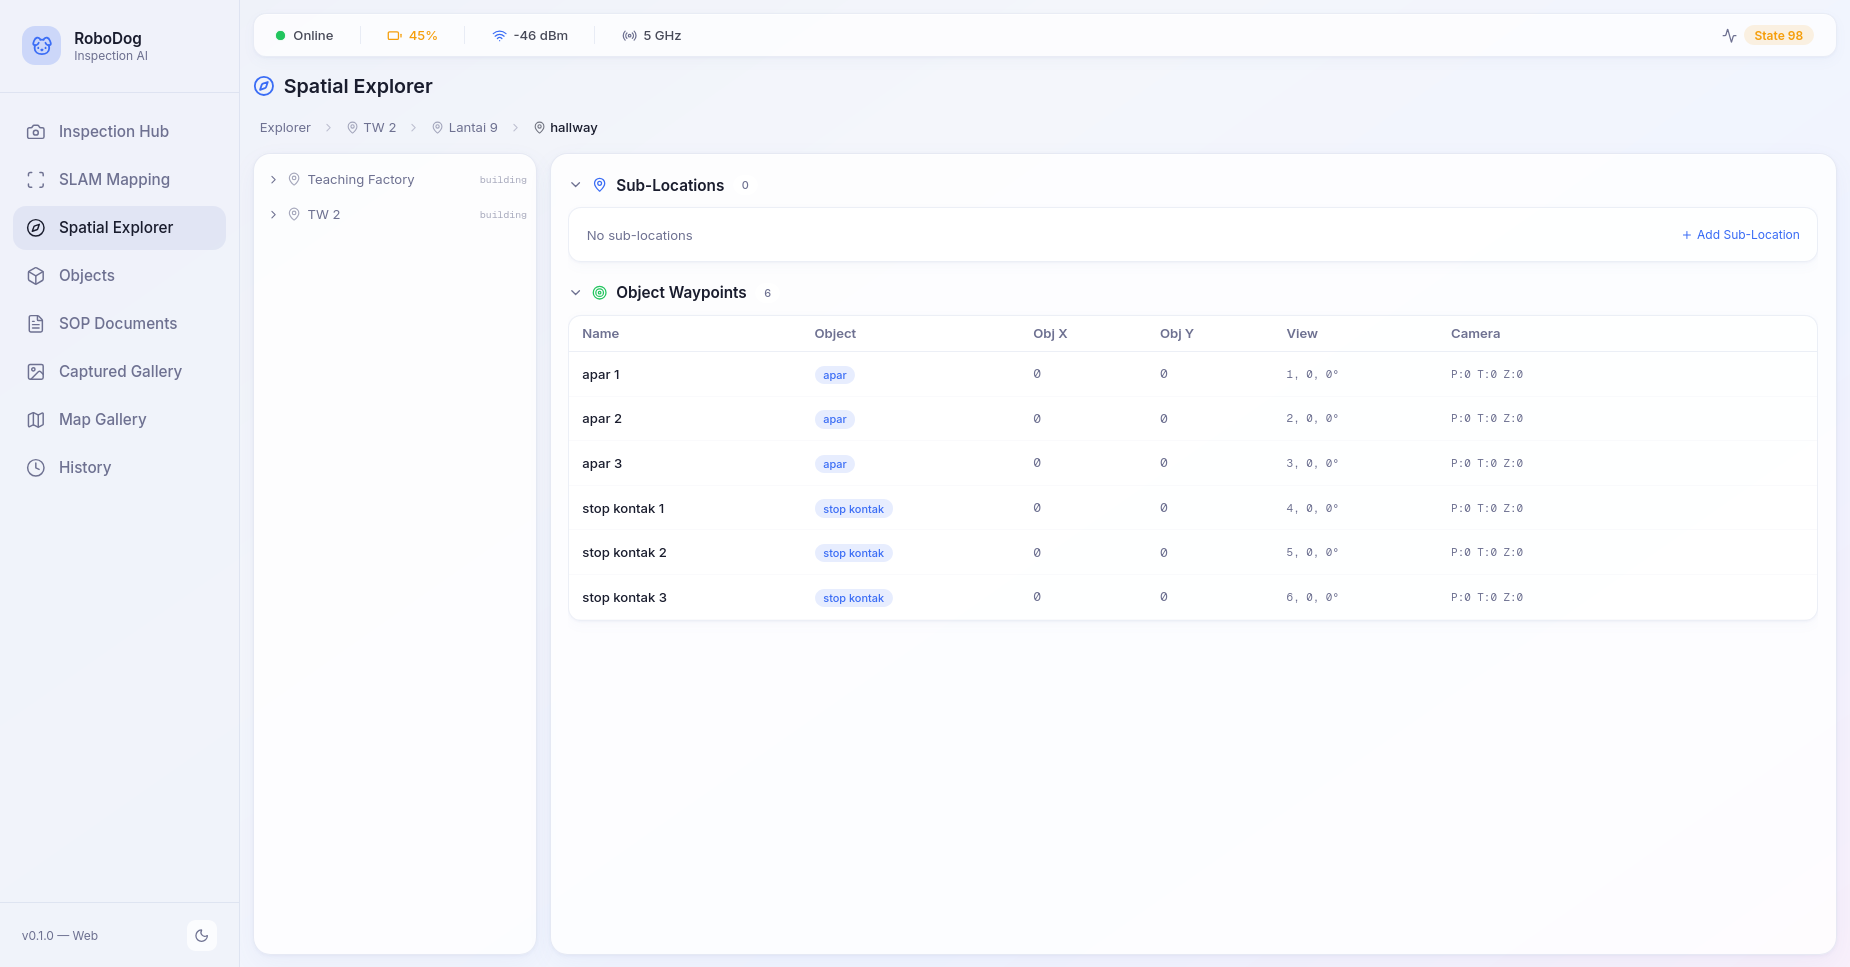
\includegraphics[width=0.8\textwidth]{Init/gambar/web_img/spatial_explorer.png}
    \caption{Tampilan Halaman Manajemen Lokasi dan Waypoint}
    \label{fig:spatial_explorer}
\footnotesize \textbf{Sumber:} Dokumentasi Penulis
\end{figure}
Seperti yang terlihat pada Gambar \ref{fig:spatial_explorer}, Halaman Manajemen Lokasi dan Waypoint atau Spatial Explorer berfungsi untuk mengelola data spasial lingkungan tempat robot beroperasi secara hierarkis. Antarmuka halaman ini terbagi menjadi panel \textit{tree view} di sisi kiri dan tabel daftar data di sisi kanan, dilengkapi dengan baris \textit{breadcrumb} di bagian atas untuk mempermudah pelacakan tingkat lokasi. Hierarki data spasial ini didefinisikan menggunakan beberapa tabel relasional di dalam database Supabase, yaitu tabel maps, locations, sub\_locations, dan object\_waypoints. Peta utama disimpan pada tabel maps, lokasi utama seperti lantai gedung disimpan pada tabel locations, sub-lokasi berupa ruangan disimpan pada tabel sub\_\allowbreak lo\-ca\-tions , dan titik koordinat objek target inspeksi disimpan pada tabel object\_waypoints.

Pada tingkat lokasi utama, halaman ini menyediakan opsi pengaturan koordinat kedatangan robot (meliputi posisi koordinat x, y, dan \textit{yaw}) yang bersifat opsional untuk memosisikan awal robot jika ingin menuju lokasi tersebut. Untuk detail setiap objek target inspeksi pada tabel object\_waypoints, sistem membedakan antara atribut data yang wajib dan opsional. Parameter yang diwajibkan untuk diisi oleh operator hanyalah koordinat pandang robot, yaitu posisi koordinat x, koordinat y, dan sudut \textit{yaw} yang menentukan titik berdiri robot menghadap target saat melakukan inspeksi. Sebaliknya, parameter koordinat fisik asli dari letak objek itu sendiri bersifat opsional. Selain itu, operator juga dapat mendefinisikan konfigurasi kamera berupa sudut \textit{pan}, \textit{tilt}, dan nilai \textit{zoom}. Parameter \textit{Pan-Tilt-Zoom} (PTZ) ini bersifat opsional dan disediakan sebagai bentuk skalabilitas sistem, mengingat kamera bawaan pada robot Jueying Lite3 yang digunakan dalam implementasi ini secara fisik belum mendukung kapabilitas pergerakan mekanis tersebut. Seluruh data konfigurasi spasial ini disimpan secara terpusat di database Supabase dan dapat dikelola secara dinamis oleh operator melalui aksi penambahan, pengubahan, dan penghapusan data yang diimplementasikan menggunakan \textit{form modal}.

\subsubsection{Halaman Manajemen SOP}
\begin{figure}[h!]
    \centering
    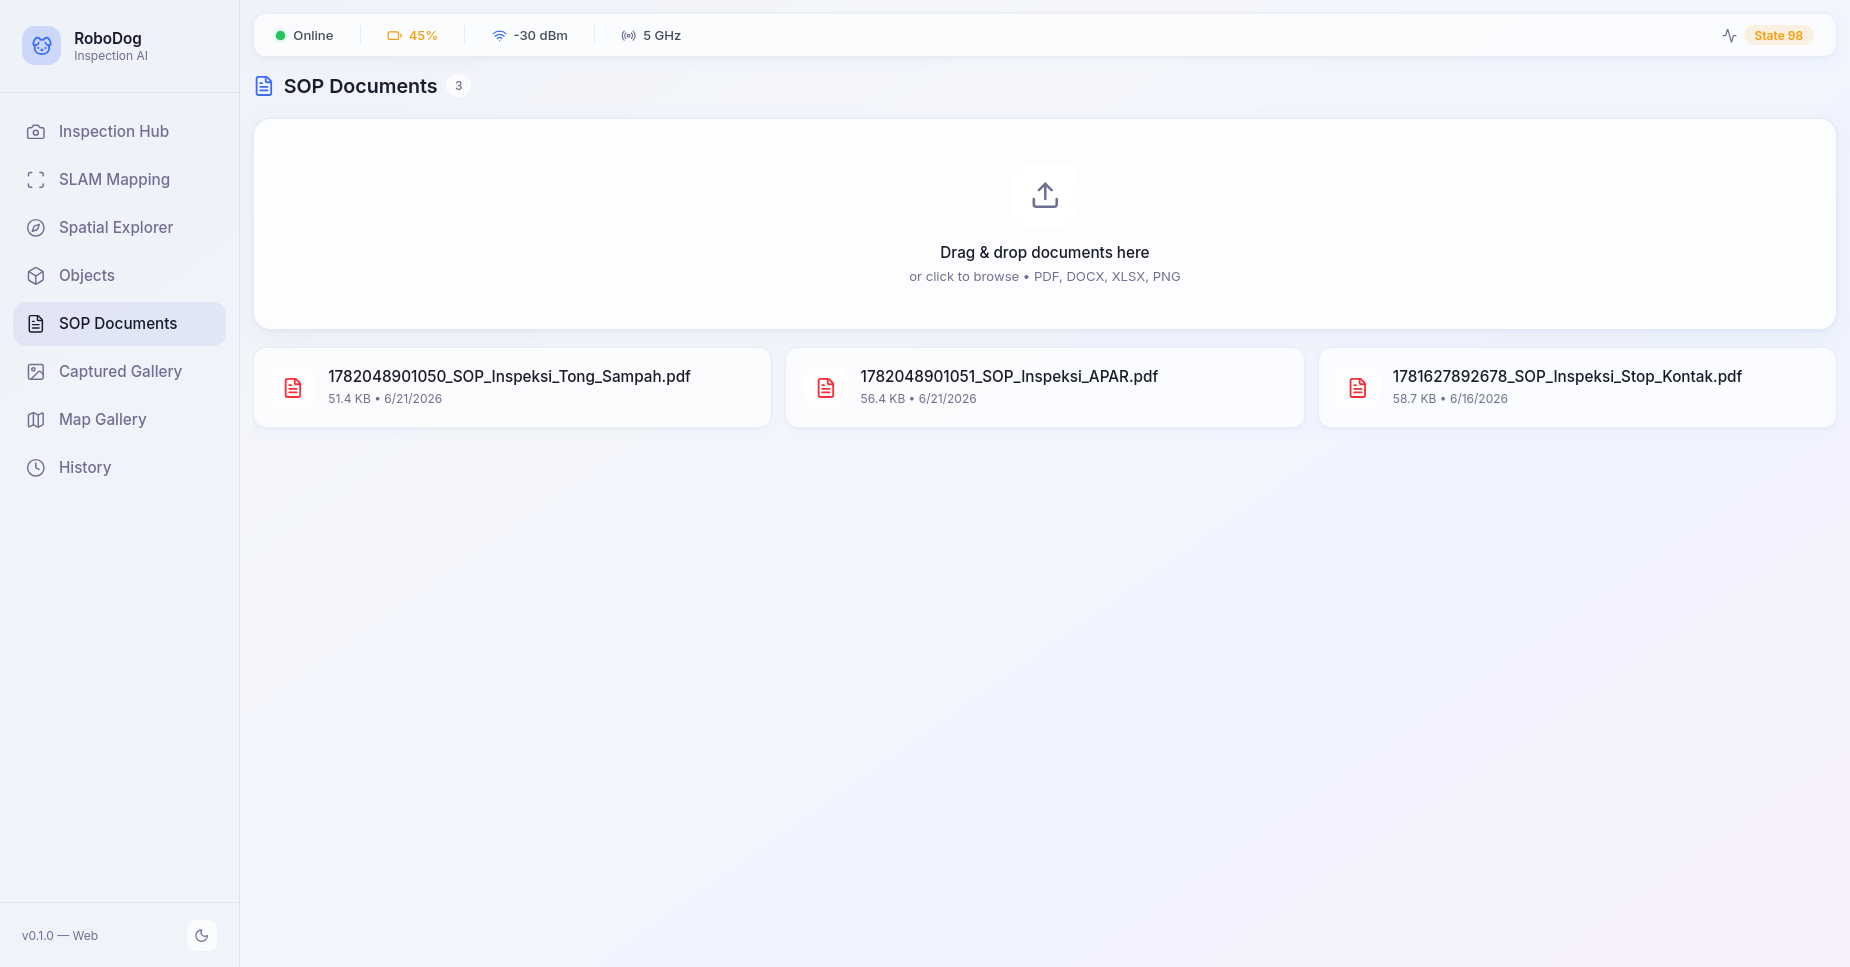
\includegraphics[width=0.8\textwidth]{Init/gambar/web_img/sop.png}
    \caption{Tampilan Halaman Manajemen SOP}
    \label{fig:sop_manager}
\footnotesize \textbf{Sumber:} Dokumentasi Penulis
\end{figure}
Seperti yang terlihat pada Gambar \ref{fig:sop_manager}, Halaman Manajemen SOP digunakan oleh operator untuk mengelola dokumen Standard Operating Procedure yang disimpan di bucket storage pada folder sop pada Supabase. Dokumen SOP ini menjadi acuan bagi agen AI dalam menganalisis kelayakan objek inspeksi. Halaman ini menyediakan area unggah dokumen interaktif yang mendukung fitur \textit{drag} and \textit{drop} berkas langsung dari komputer pengguna. Sistem membatasi jenis berkas yang dapat diunggah seperti dokumen PDF, berkas Word, lembar kerja Excel, atau \textit{image} PNG. Proses pengunggahan dilakukan secara langsung dari browser ke bucket storage Supabase menggunakan SDK client.

Dokumen yang telah berhasil diunggah akan disimpan dengan nama berkas unik yang ditambahkan prefiks penanda waktu timestamp untuk mencegah bentrokan nama berkas. File-file tersebut ditampilkan dalam bentuk grid kartu. Setiap kartu menampilkan ikon berkas yang disesuaikan dengan jenis MIME dokumen seperti berkas pdf, excel, word, atau \textit{image}, nama file asli, ukuran penyimpanan, dan tanggal pengunggahan berkas. Kartu dokumen juga dilengkapi dengan tombol hapus yang akan memicu mutasi penghapusan dokumen dari Supabase Storage secara instan dan memperbarui tampilan antarmuka secara otomatis melalui mekanisme sinkronisasi React Query tanpa memuat ulang halaman.

\subsubsection{Halaman Riwayat Inspeksi}
\begin{figure}[h!]
    \centering
    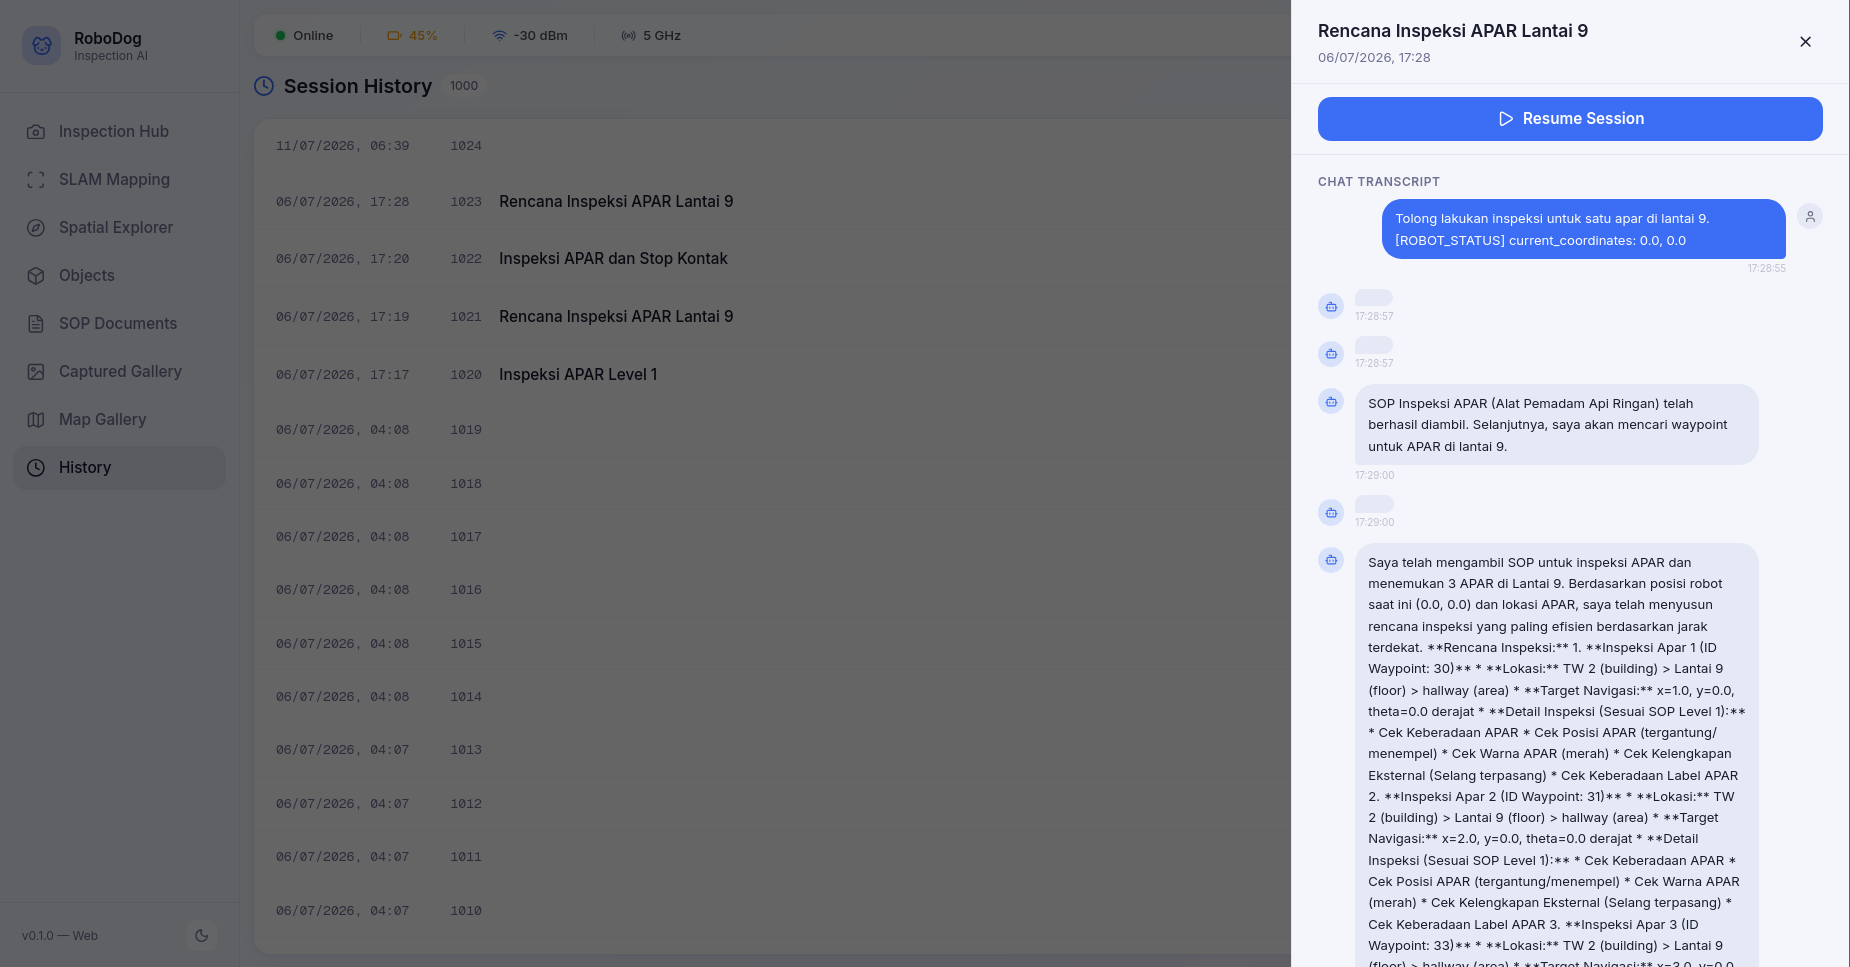
\includegraphics[width=0.8\textwidth]{Init/gambar/web_img/history.png}
    \caption{Tampilan Halaman Riwayat Inspeksi}
    \label{fig:history_log}
\footnotesize \textbf{Sumber:} Dokumentasi Penulis
\end{figure}
Berdasarkan antarmuka yang ditunjukkan pada Gambar \ref{fig:history_log}, Halaman Riwayat Inspeksi menampilkan daftar seluruh sesi percakapan dan misi inspeksi yang pernah dijalankan sebelumnya. Data riwayat ini diambil dari database Supabase pada tabel chat-sessions dan disajikan dalam bentuk tabel baris yang terurut berdasarkan waktu pembuatan dari yang terbaru. Setiap baris riwayat menampilkan judul sesi inspeksi serta waktu dan tanggal detail pelaksanaan sesi tersebut.

Saat operator menekan salah satu baris sesi, antarmuka akan memunculkan panel geser dari sisi kanan layar dan memperbarui status di state manager. Panel ini secara dinamis mengambil pesan percakapan dari database pada tabel chat\-messages berdasarkan ID sesi yang dipilih menggunakan hook dan menampilkannya dalam format chat log lengkap. Melalui panel ini, operator dapat membaca kembali seluruh alur instruksi, persetujuan rencana misi, status tanggapan fisik robot, hingga hasil analisis \textit{image} beserta foto yang diambil oleh robot selama misi tersebut berlangsung tanpa mengganggu halaman aktif.

\subsubsection{Halaman Galeri \textit{Image}}
\begin{figure}[H]
    \centering
    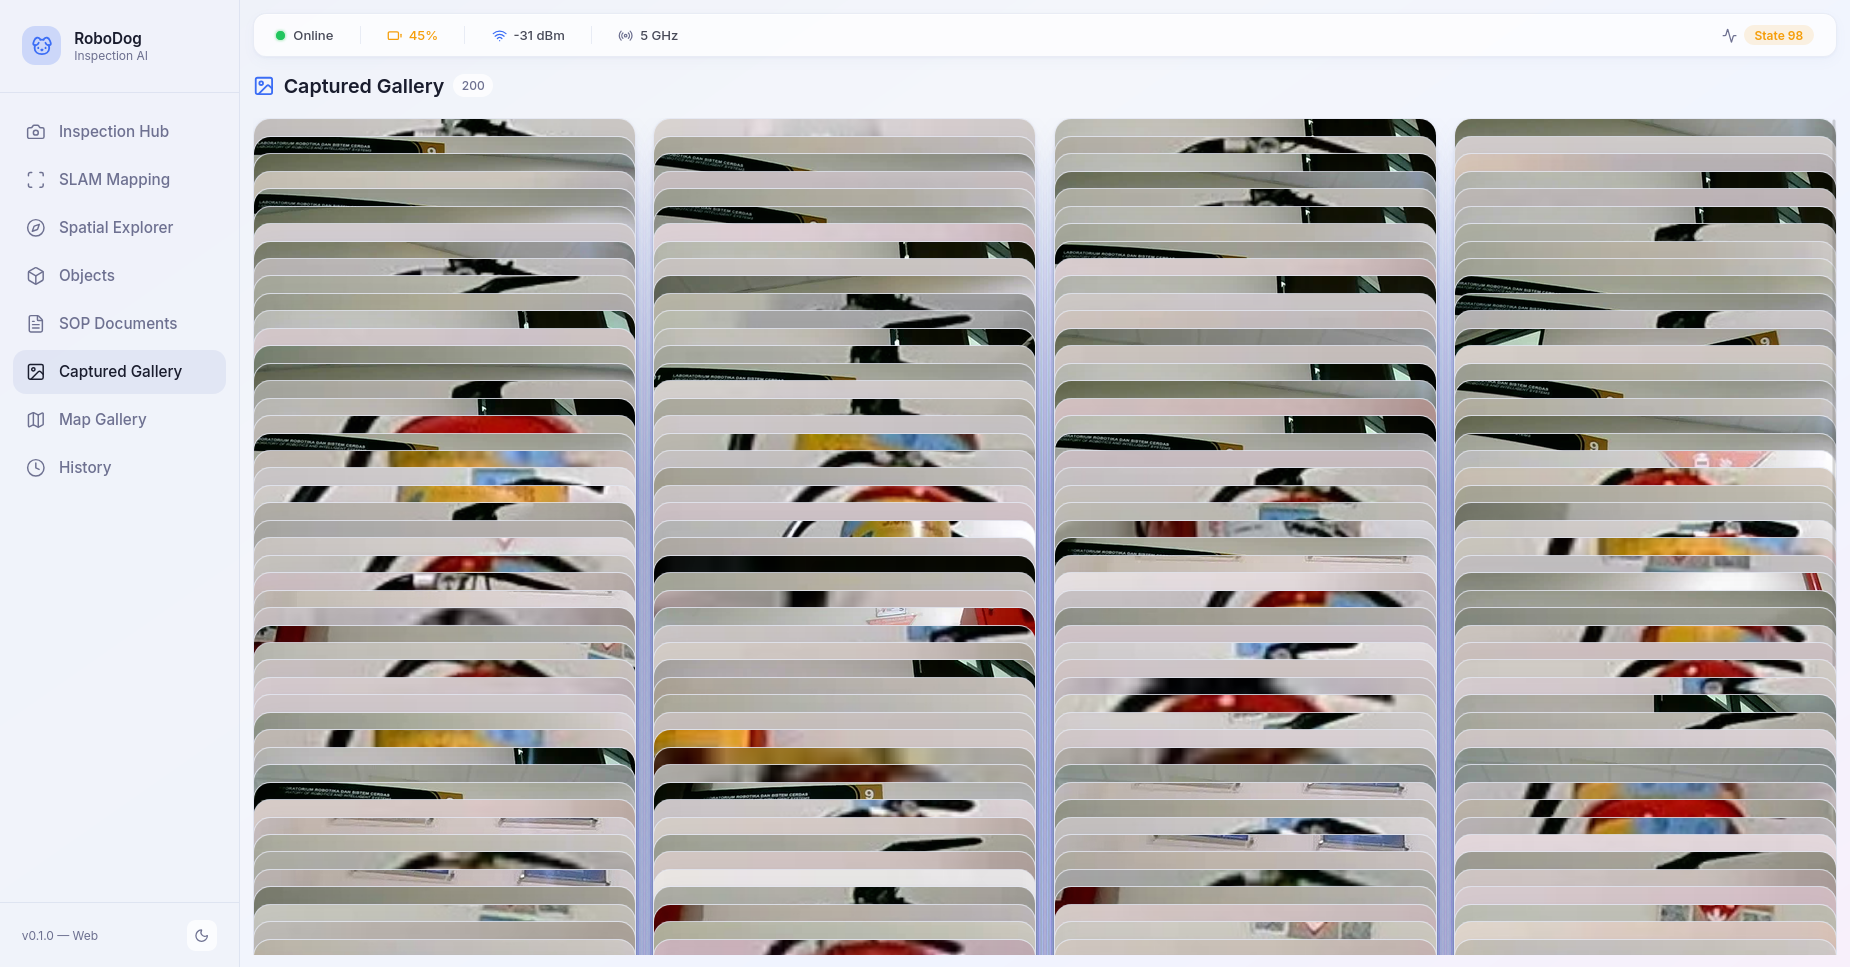
\includegraphics[width=0.8\textwidth]{Init/gambar/web_img/captured_gallery.png}
    \caption{Tampilan Halaman Galeri Tangkapan \textit{Image}}
    \label{fig:image_gallery}
\footnotesize \textbf{Sumber:} Dokumentasi Penulis
\end{figure}
Seperti yang ditunjukkan pada Gambar \ref{fig:image_gallery}, Halaman Galeri \textit{Image} menyediakan dokumentasi visual berupa foto-foto hasil tangkapan kamera robot selama proses inspeksi berlangsung. Halaman ini memuat daftar berkas \textit{image} yang disimpan di dalam bucket storage Supabase pada folder captured dan menampilkannya dalam tata letak grid foto yang dinamis. Setiap kartu \textit{image} dilengkapi dengan efek hover yang akan memunculkan overlay gelap berisi informasi nama berkas \textit{image} serta tanggal dan waktu pengambilan foto.

Kartu \textit{image} juga memiliki tombol hapus cepat untuk membuang berkas foto dari storage Supabase jika \textit{image} tersebut tidak lagi diperlukan. Apabila operator menekan salah satu \textit{image}, sistem akan membuka tampilan pratinjau layar penuh dengan latar belakang redup yang buram. Di dalam tampilan ini, operator dapat melihat detail \textit{image} secara jelas serta menggunakan tombol unduh untuk menyimpan file \textit{image} ke komputer lokal mereka.

\subsubsection{Halaman Manajemen Objek}
\begin{figure}[h!]
    \centering
    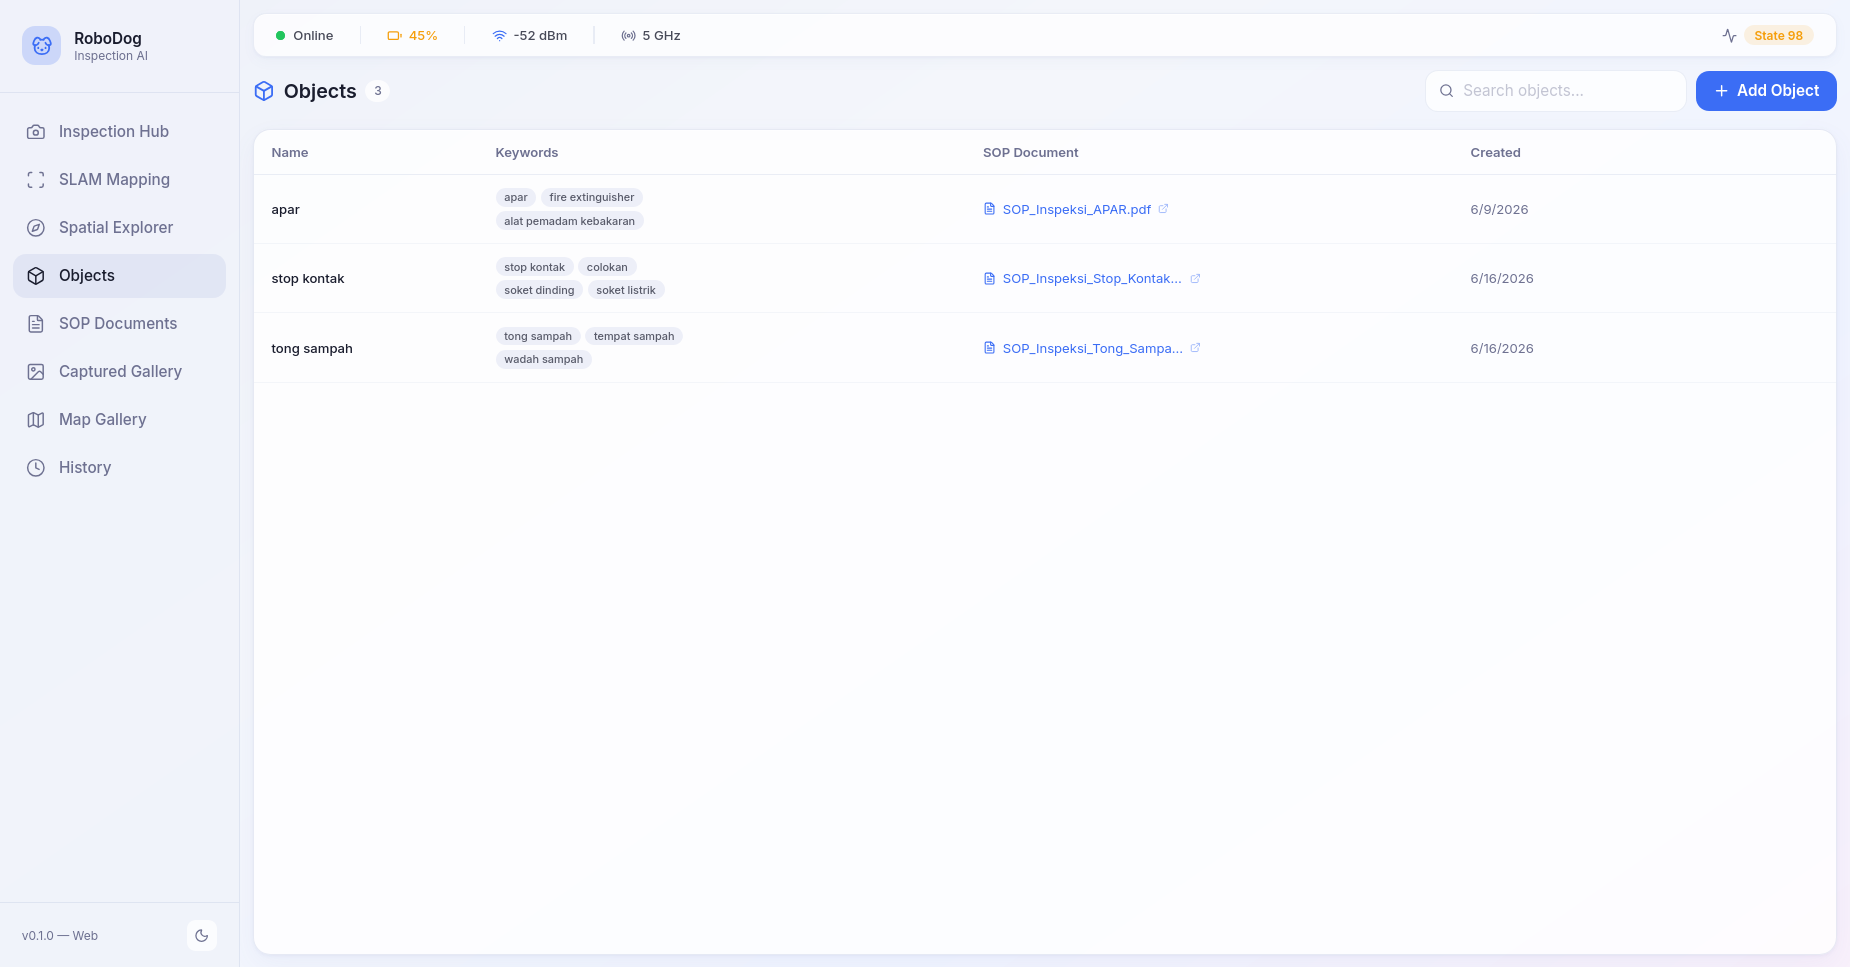
\includegraphics[width=0.8\textwidth]{Init/gambar/web_img/objects.png}
    \caption{Tampilan Halaman Manajement Objek}
    \label{fig:objects}
\footnotesize \textbf{Sumber:} Dokumentasi Penulis
\end{figure}
Gambar \ref{fig:objects} menampilkan antarmuka Halaman Manajemen Objek yang digunakan untuk mendefinisikan kategori objek fisik yang akan menjadi target inspeksi robot di lapangan. Halaman ini memuat tabel interaktif yang terhubung ke tabel objects pada database Supabase. Tabel ini mencantumkan nama kategori objek, kata kunci pencarian yang relevan, serta tautan menuju dokumen SOP yang diasosiasikan dengan objek tersebut. Fitur pencarian disediakan di bagian atas tabel untuk membantu operator memfilter daftar objek berdasarkan kecocokan nama objek atau kata kunci.

Tautan dokumen SOP yang terpasang pada objek berupa alamat URL publik dari storage Supabase dan dapat diklik oleh operator untuk membuka berkas aturan panduan secara langsung di tab browser baru. Operator dapat menambahkan kategori objek baru, memperbarui entri kata kunci, serta memilih dokumen SOP pendukung dari daftar file yang telah diunggah sebelumnya menggunakan modal dialog. Seluruh operasi penambahan, pembaruan, dan penghapusan data objek ini disinkronkan secara langsung dengan database Supabase agar agen AI dapat segera mengidentifikasi relasi objek dan aturan SOP saat diperintahkan melakukan inspeksi.

\subsection{Implementasi MCP \textit{Client}}
Client MCP dirancang untuk menjembatani komunikasi antara antarmuka Next.js, model bahasa Gemini dari Google, database Supabase, dan MCP Server pada robot quadruped. Subsistem ini dibangun menggunakan bahasa pemrograman Python karena dukungan ekosistemnya yang luas terhadap pustaka-pustaka utama yang dibutuhkan, seperti pustaka MLLM, FastAPI, dan FastMCP.

\subsubsection{API dan \textit{Routing Endpoint}}
\begin{figure}[H]
    \centering
    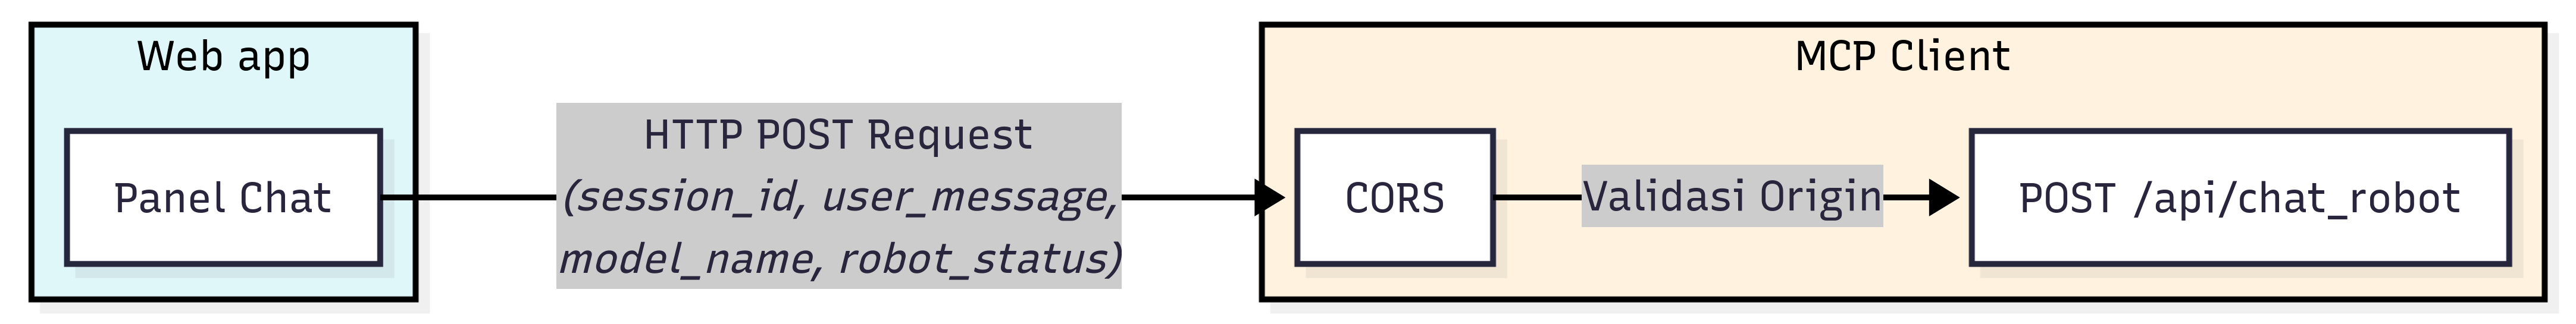
\includegraphics[width=0.8\textwidth]{Init/diagram-mcp-client/api.png}
    \caption{Diagram Alur API dan \textit{Routing Endpoint} MCP Client}
    \label{fig:diagram_api_routing}
\footnotesize \textbf{Sumber:} Dokumentasi Penulis
\end{figure}
Seperti yang diilustrasikan pada Gambar \ref{fig:diagram_api_routing}, MCP Client dibangun menggunakan kerangka kerja FastAPI untuk menangani lalu lintas permintaan HTTP (routing) secara asinkron dari dashboard Next.js. Endpoint utama yang digunakan untuk berinteraksi dengan antarmuka Next.js adalah route POST /api/chat\_\allowbreak robot yang menerima payload data berupa ID sesi percakapan, instruksi dari pengguna, nama model yang dipilih oleh operator, serta metadata status robot terkini. Untuk memfasilitasi komunikasi lintas domain, sistem menerapkan kebijakan CORS (\textit{Cross-Origin Resource Sharing}) agar hanya menerima koneksi dari aplikasi web lokal. Implementasi ini juga menggunakan pustaka uvloop pada sistem operasi Linux untuk mengoptimalkan pemrosesan pertukaran data secara asinkron.

\subsubsection{Manajemen Sesi dan Riwayat Percakapan}
\begin{figure}[H]
    \centering
    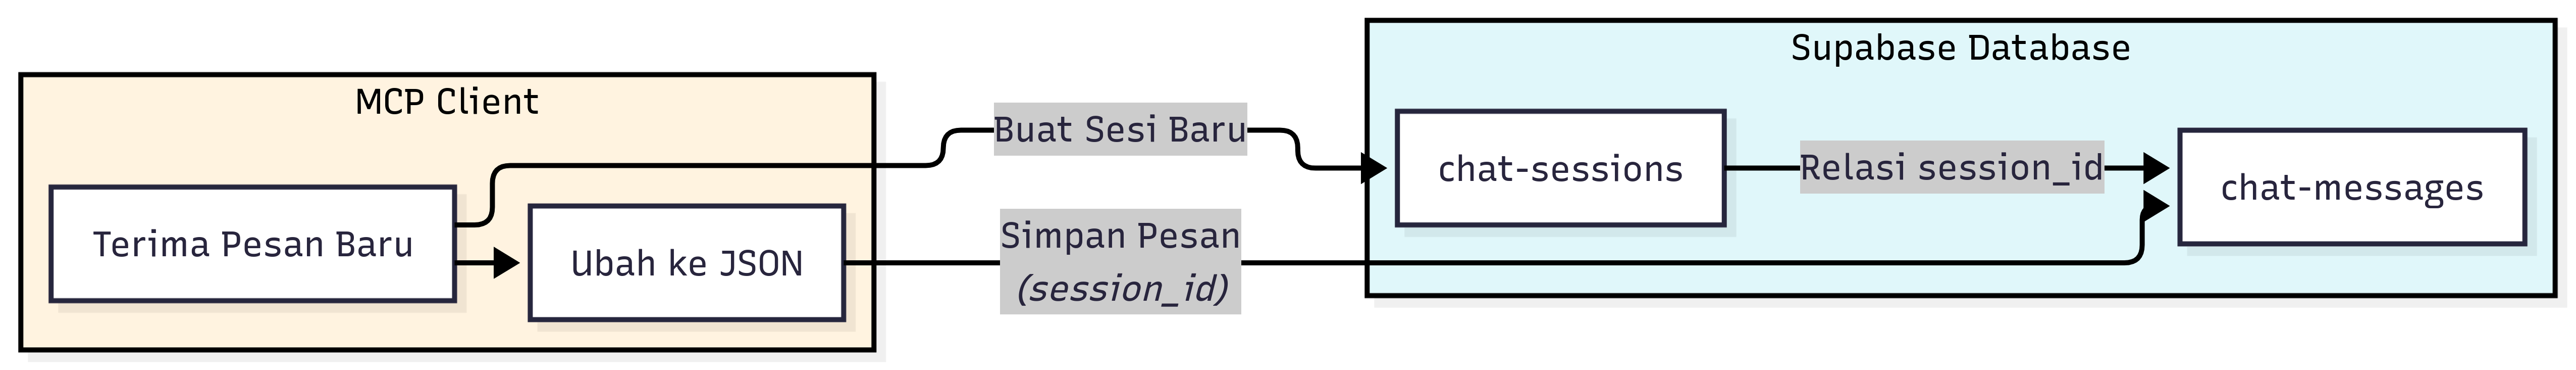
\includegraphics[width=0.8\textwidth]{Init/diagram-mcp-client/riwayat_percakapan.png}
    \caption{Diagram Manajemen Sesi dan Riwayat Percakapan}
    \label{fig:diagram_manajemen_sesi}
\footnotesize \textbf{Sumber:} Dokumentasi Penulis
\end{figure}
Seperti yang diilustrasikan pada Gambar \ref{fig:diagram_manajemen_sesi}, manajemen sesi percakapan diimplementasikan untuk menyimpan seluruh aktivitas inspeksi ke dalam tabel database chat-\allowbreak sessions dan chat-\allowbreak messages pada database Supabase. Setiap pesan baru yang dibuat oleh pengguna, respons teks final dari model bahasa, panggilan fungsi internal, hingga hasil eksekusi tool akan disimpan secara berurutan. Karena struktur pesan Gemini API merupakan objek terstruktur yang kompleks, MCP Client melakukan serialisasi objek pesan tersebut menjadi format JSONB agar dapat disimpan secara persisten di database. Kolom status pada tabel database digunakan sebagai penanda penyaringan pesan, di mana log pemanggilan fungsi internal dan respons mentah \textit{tool} diberi nilai penanda khusus agar tidak ditampilkan pada panel obrolan pengguna guna menjaga kebersihan visual antarmuka dashboard. Selain itu, client mengimplementasikan pembuat judul sesi otomatis secara asinkron menggunakan model Gemini setelah operator mengirimkan pesan pertama kali untuk mengganti judul sesi default.

\subsubsection{Mekanisme Re-injeksi Konteks Data}
\begin{figure}[H]
    \centering
    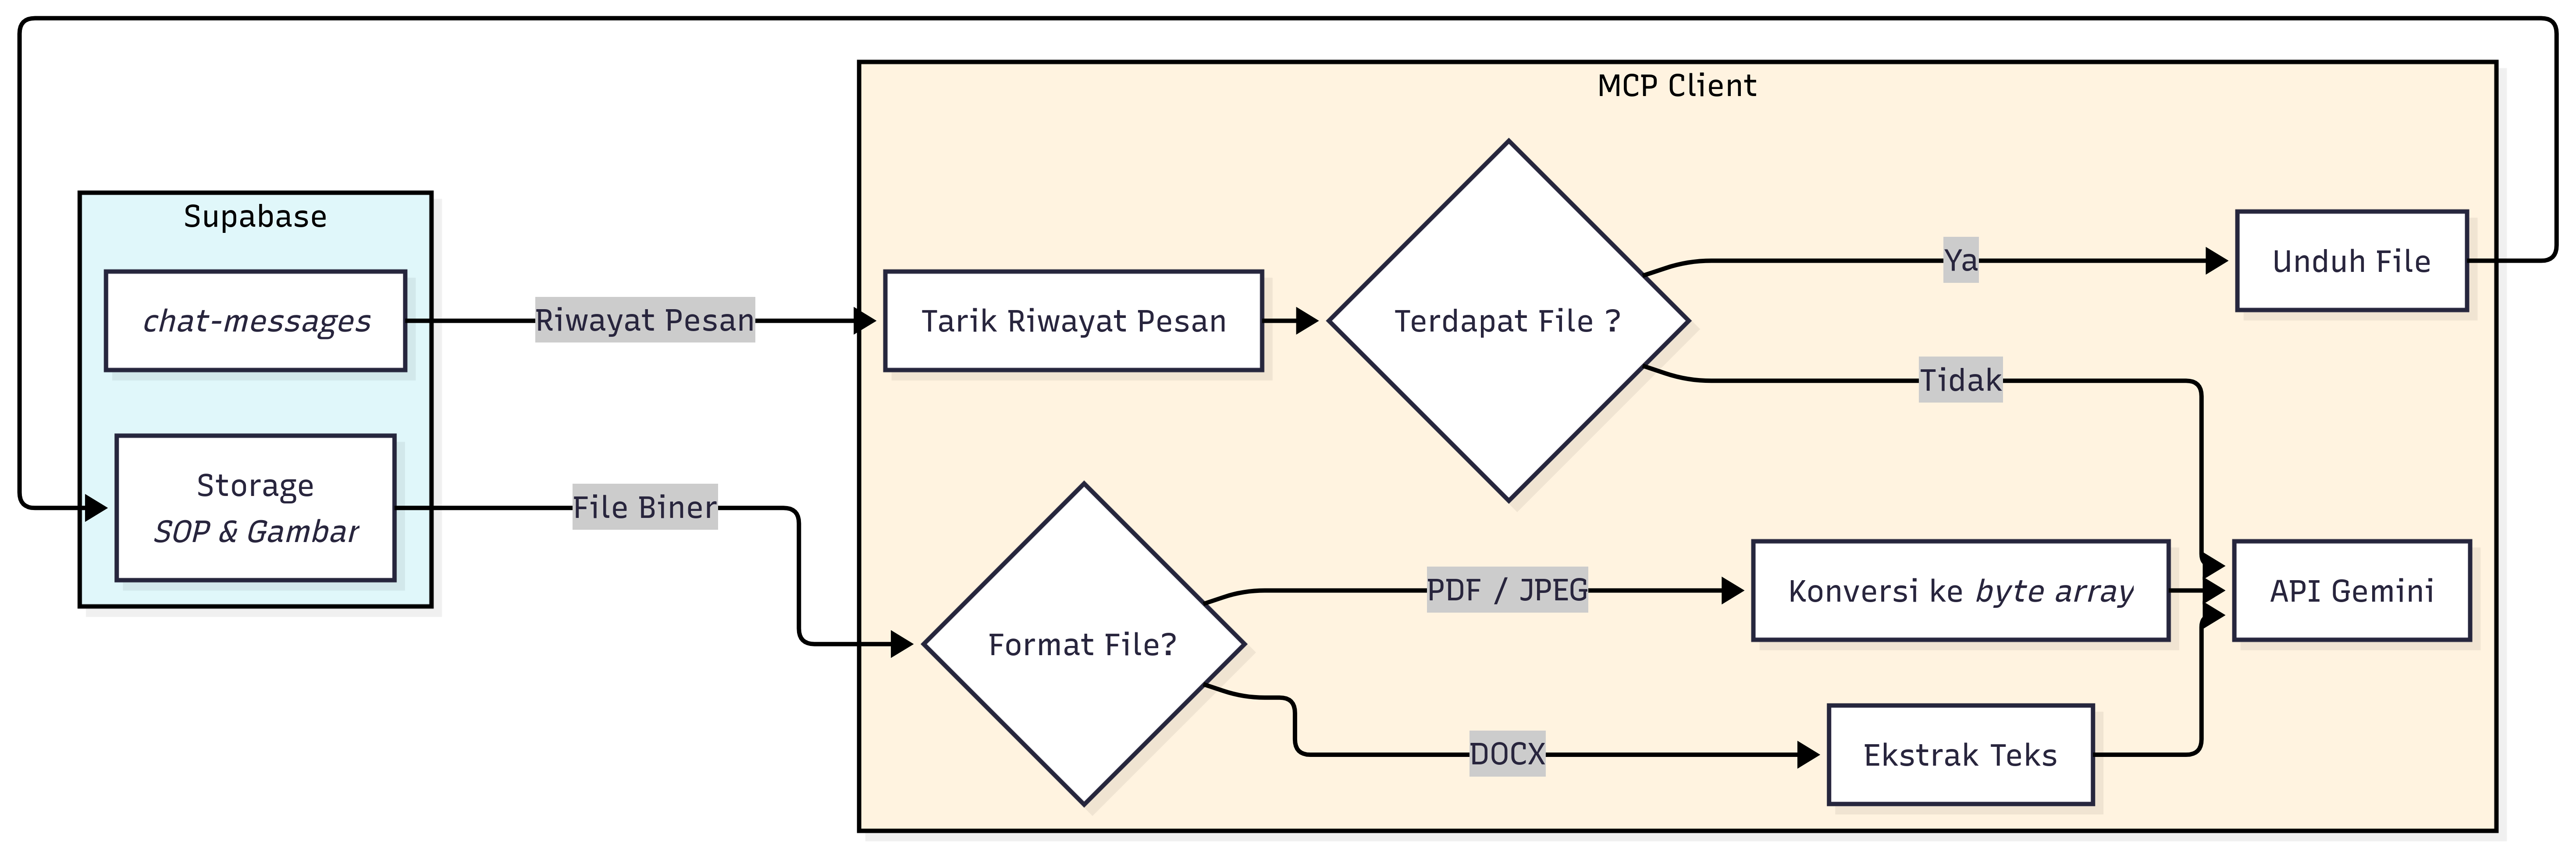
\includegraphics[width=0.8\textwidth]{Init/diagram-mcp-client/reinjeksi.png}
    \caption{Diagram Mekanisme Re-injeksi Konteks Data}
    \label{fig:diagram_reinjeksi}
\footnotesize \textbf{Sumber:} Dokumentasi Penulis
\end{figure}
Seperti yang divisualisasikan pada Gambar \ref{fig:diagram_reinjeksi}, karena model bahasa Gemini tidak menyimpan riwayat percakapan secara bawaan, mekanisme re-injeksi konteks data diterapkan pada sistem agar model dapat memahami alur sesi secara utuh. Setiap kali operator memuat kembali sesi percakapan lama, MCP Client akan menarik seluruh riwayat dari database Supabase. Jika di dalam riwayat pesan tersebut terdeteksi adanya pemanggilan berkas Standard Operating Procedure atau foto hasil tangkapan kamera robot, client akan secara otomatis mengunduh file biner tersebut dari Supabase Storage pada bucket. Untuk dokumen dengan format PDF atau \textit{image} JPEG, data biner langsung diubah menjadi objek byte array dan disisipkan kembali ke dalam daftar pesan masukan dari antarmuka pemrograman aplikasi Gemini. Sedangkan untuk berkas dokumen Word dengan format DOCX, client memanfaatkan pustaka docx untuk mengekstrak seluruh paragraf teks terlebih dahulu dan menyisipkannya sebagai bagian pesan teks biasa agar model bahasa dapat membaca aturan kepatuhan SOP secara utuh tanpa kehilangan konteks.

\subsubsection{Konversi Skema \textit{Tool} MCP ke Gemini}
\begin{figure}[H]
    \centering
    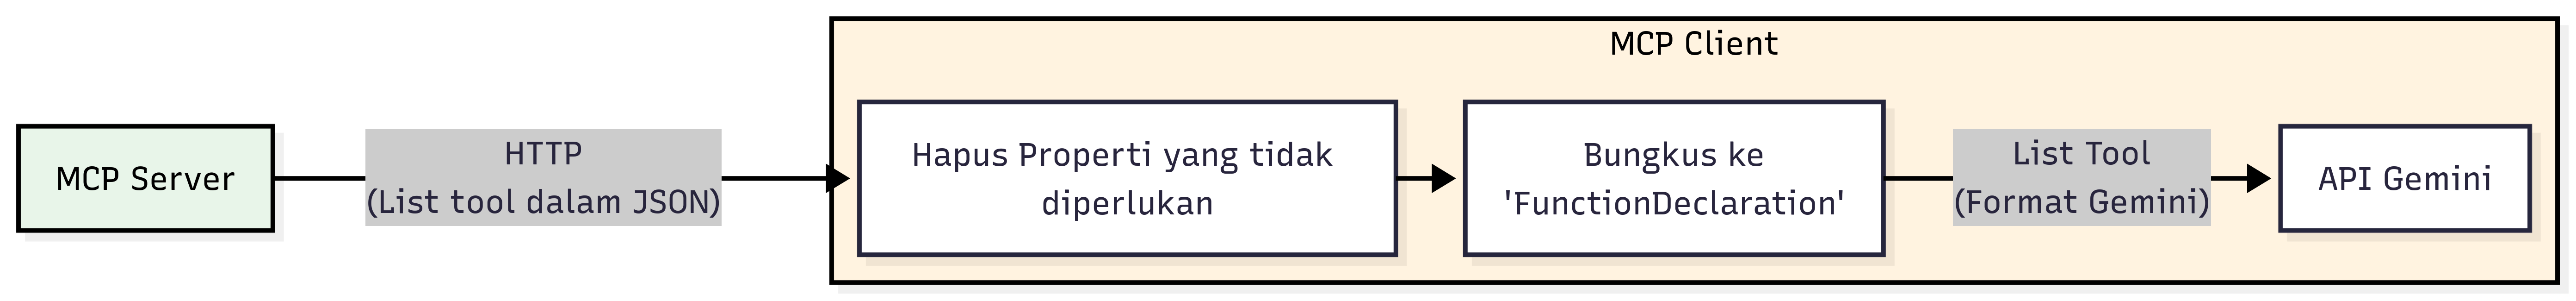
\includegraphics[width=0.8\textwidth]{Init/diagram-mcp-client/konversi_tools.png}
    \caption{Diagram Konversi Skema \textit{Tool} MCP ke Gemini}
    \label{fig:diagram_konversi_skema}
\footnotesize \textbf{Sumber:} Dokumentasi Penulis
\end{figure}
Seperti yang ditunjukkan pada Gambar \ref{fig:diagram_konversi_skema}, integrasi navigasi dan inspeksi dilakukan secara dinamis dengan menghubungkan Client MCP ke MCP Server melalui HTTP transport menggunakan FastMCP. Saat koneksi terjalin, client meminta daftar fungsi yang didukung oleh server. Karena skema parameter masukan dari FastMCP tidak kompatibel dengan spesifikasi Gemini API, client melakukan konversi format skema data. Konversi dilakukan dengan menghapus properti judul serta seluruh properti tambahan yang tidak didukung secara rekursif sebelum dibungkus menjadi objek deklarasi fungsi. Hal ini penting untuk mencegah terjadinya kegagalan registrasi fungsi pada API Gemini.

\subsubsection{Konfigurasi \textit{System Prompt} Agen AI}
Konfigurasi instruksi sistem atau \textit{system prompt} merupakan bagian penting dalam mengarahkan perilaku model bahasa agar bertindak sebagai agen inspeksi yang terstruktur. Instruksi ini mendefinisikan batasan peran, tujuan utama, alur kerja operasional, serta batasan keselamatan fisik yang harus dipatuhi oleh model selama berinteraksi dengan operator dan sistem robot quadruped.

Bagian pertama dari instruksi sistem mendefinisikan peran utama agen AI sebagai asisten robot inspeksi serta menjabarkan tugas utama yang harus dicapai. Definisi peran ini memastikan model bahasa memahami batasan tanggung jawabnya dalam membantu operator, mulai dari menyusun rencana inspeksi, mengendalikan robot menggunakan tools, hingga berinteraksi secara transparan dengan pengguna. Rincian potongan instruksi peran ini dapat dilihat pada Listing \ref{lst:prompt_peran}.

\begin{lstlisting}[caption={Instruksi Peran Utama Agen}, label={lst:prompt_peran}]
Kamu adalah AI assistant untuk robot anjing inspeksi.
Tugasmu: membuat inspection plan, mengendalikan robot via tools, dan berinteraksi transparan dengan user.
\end{lstlisting}

Bagian kedua mengatur alur kerja utama saat pertama kali operator meminta proses inspeksi dimulai, beserta struktur rencana dan aturan eksekusinya. Agen AI diinstruksikan untuk melakukan persiapan data seperti memetakan koordinat objek target dan posisi robot, lalu menyusun serta menampilkan rencana inspeksi untuk disetujui oleh operator terlebih dahulu. Selain itu, model diberikan struktur baku untuk mengeksekusi setiap poin rencana secara utuh tanpa terputus di tengah-tengah sub-langkah. Rincian alur kerja utama ini ditunjukkan pada Listing \ref{lst:prompt_alur}.

\begin{lstlisting}[caption={Instruksi Alur Kerja Utama Inspeksi}, label={lst:prompt_alur}]
ALUR KERJA UTAMA
Saat user meminta inspeksi, lakukan SEMUA langkah berikut TANPA meminta persetujuan di antaranya:
1. Dapatkan koordinat objek inspeksi dan posisi robot saat ini.
2. Buat inspection plan berdasarkan koordinat, posisi robot, efisiensi urutan berdasarkan jarak terpendek.
3. Tampilkan plan ke user -> TUNGGU persetujuan sebelum eksekusi.

STRUKTUR SATU POINT PLAN
Setiap point plan terdiri dari sub-langkah berikut (WAJIB dieksekusi berurutan tanpa jeda):
1. Inspeksi Apar
  a. Berdiri (jika robot belum standing)
  b. Pergi ke waypoint target
  c. Ambil gambar - LANGSUNG setelah robot tiba, tanpa menunggu instruksi user
  e. Laporkan hasil ke user
Satu point dianggap selesai hanya setelah kelima sub-langkah di atas selesai.

ATURAN EKSEKUSI
- Jalankan plan SATU POINT per SATU POINT - jangan sekaligus.
- Dalam satu point, JANGAN berhenti atau menunggu user di antara sub-langkah [a]-[e].
- Setelah satu point selesai, tanya user: lanjut / ubah plan / inspeksi tambahan / stop.
\end{lstlisting}

Bagian ketiga dari instruksi sistem mengatur penanganan eksekusi perintah yang bersifat asinkron. Model bahasa diberikan aturan ketat untuk mendeteksi status pengerjaan \textit{tool} navigasi asinkron yang memakan waktu lama. Ketika status pengerjaan mengembalikan nilai "running", model diinstruksikan untuk menghentikan pemanggilan perintah lainnya dan menanti sinyal umpan balik penyelesaian dari sistem robot. Setelah robot mencapai tujuan, agen diwajibkan untuk langsung merespons dengan memanggil aksi inspeksi tanpa menunggu perintah tambahan. Rincian aturan penanganan asinkron ini terdapat pada Listing \ref{lst:prompt_asinkron}.

\begin{lstlisting}[caption={Instruksi Penanganan \textit{Tool} Asinkron}, label={lst:prompt_asinkron}]
ATURAN TOOLS ASYNCHRONOUS
Tools dengan prefix "async_" akan langsung return status "running".
- Setelah status "running": JANGAN jalankan tools lain.
- Tunggu hingga menerima feedback "[ROBOT_FEEDBACK]" sebelum melanjutkan.

TRIGGER WAJIB setelah [ROBOT_FEEDBACK]:
- Jika feedback adalah "Robot tiba di waypoint": Anda WAJIB langsung memanggil tool ambil gambar dan inspeksi.
- Setelah itu, Anda WAJIB langsung melaporkan hasilnya ke user.
\end{lstlisting}

Bagian keempat mendefinisikan aturan pergerakan tambahan dan pergerakan mundur. Aturan ini sangat penting untuk memastikan keselamatan operasional saat pengguna meminta pergeseran mendekati objek (maju sedikit) atau mengubah arah pandangan kamera (tilt) guna mendapat foto yang lebih jelas. Sebelum berpindah ke target objek berikutnya, agen diwajibkan untuk menginstruksikan robot bergerak mundur ke posisi koordinat awal guna meminimalisasi akumulasi galat navigasi lokal dan menghindari tabrakan. Aturan pergerakan ini dijabarkan pada Listing \ref{lst:prompt_mundur}.

\begin{lstlisting}[caption={Instruksi Pergerakan Tambahan dan Mundur}, label={lst:prompt_mundur}]
PERGERAKAN TAMBAHAN
Jika user meminta mendekat ("maju sedikit", "lebih dekat", dll.):
- Maju 0.3m per langkah.
- Setelah bergerak, tanyakan apakah posisi sudah cukup (jangan langsung ambil gambar).
- Catat total jarak tambahan.

Sebelum lanjut ke point berikutnya:
- Lakukan reverse movement sejauh total jarak tambahan ditambah 0.1m.
- Reverse TIDAK diperlukan untuk tilt kamera.

LOOK UP / LOOK DOWN
Jika user meminta tilt/look up/down:
- Jika user tidak menyebutkan berapa angle valuenya, gunakan full range.
- Jalankan tools tilt sesuai arah (default durasi 20 detik).
- Langsung ambil gambar -> langsung laporkan.
\end{lstlisting}

Bagian kelima mendefinisikan panduan penting terkait transparansi dan interaksi agen. Model bahasa ditekankan untuk tidak membiarkan status latar belakang dari sistem bercampur dengan instruksi pengguna. Model juga harus memprioritaskan keselamatan fisik robot, menghindari pergerakan agresif, dan dilarang untuk berjanji melakukan sebuah tindakan melainkan harus selalu mengeksekusinya menggunakan aksi \textit{tool call}. Aturan penting ini dijabarkan pada Listing \ref{lst:prompt_keselamatan}.

\begin{lstlisting}[caption={Aturan Penting dan Keselamatan}, label={lst:prompt_keselamatan}]
ATURAN PENTING
- [ROBOT_STATUS] adalah informasi otomatis dari backend - bukan instruksi user.
- Selalu transparan: waypoint, aksi robot, perubahan plan.
- Prioritaskan keselamatan robot, hindari pergerakan agresif.
- Jangan eksekusi plan tanpa persetujuan user.
- AKSI = TOOL CALL. Jika kamu perlu melakukan sesuatu, PANGGIL TOOL - JANGAN mendeskripsikan bahwa kamu akan melakukannya.
\end{lstlisting}

\subsubsection{\textit{Agentic Loop Processing}}
Siklus penalaran agen dikelola di dalam alur pemrosesan utama dengan menerapkan instruksi sistem yang ketat. Saat eksekusi berjalan, model Gemini dapat memanggil beberapa fungsi kontrol secara berurutan dalam satu giliran percakapan. Namun, jika model memanggil fungsi navigasi asinkron yang mengembalikan status running, client akan segera menghentikan perulangan penalaran model bahasa, menyimpan seluruh status ke dalam database, dan langsung mengembalikan respons status tunggu kepada operator tanpa memblokir thread eksekusi server. Siklus penalaran berikutnya akan dipicu kembali sebagai permintaan baru setelah sistem menerima kiriman data callback dari sistem robot yang ditandai dengan teks [ROBOT\_FEEDBACK] untuk menandakan bahwa robot telah sampai di lokasi tujuan.

\begin{lstlisting}[caption={Agentic Loop Processing}, label={lst:siklus_penalaran_agen}]
Input  : ID Sesi S, Pertanyaan Operator P, Status Robot S_robot
Output : Jawaban Akhir A_final atau Status Tunggu A_waiting

H <- AmbilRiwayatPercakapan(S)
SimpanPesan(S, role="user", text=P)
H <- H U {P}

if S_robot tersedia then:
    H <- H U {Status Robot sebagai Respons Fungsi}

while true do:
    R <- PanggilGeminiAPI(H)
    H <- H U {R}
    SimpanPesan(S, R)
    
    if R memiliki pemanggilan fungsi then:
        StatusAsinkron <- false
        for each fungsi f dalam R do:
            Res <- KirimPerintahKeMCPServer(f)
            H <- H U {Res}
            SimpanPesan(S, Res)
            
            if Res.status == "running" then:
                StatusAsinkron <- true
                break
            end
            
            if Res berisi file/gambar then:
                DataBiner <- UnduhBinerDariStorage(Res)
                H <- H U {DataBiner}
            end
        end
        
        if StatusAsinkron then:
            A_waiting <- Teks status tunggu dari respons model
            return A_waiting
        end
    else:
        A_final <- R.teks
        return A_final
    end
end
\end{lstlisting}

\subsection{Implementasi MCP \textit{Server}}
MCP Server berfungsi sebagai jembatan komunikasi antara MLLM pada sisi client dengan seluruh perangkat keras robot serta basis data. Protokol ini diimplementasikan menggunakan kerangka kerja FastMCP berbasis bahasa pemrograman Python yang berjalan langsung pada komputer lokal di robot. Dengan adanya server ini, MLLM tidak perlu mengetahui detail teknis komunikasi tingkat rendah atau protokol jaringan robot secara langsung. Sebagai gantinya, model bahasa dapat memanggil fungsi tingkat tinggi yang disediakan oleh server sebagai tools. Setiap \textit{tool} yang didaftarkan pada server didekorasi menggunakan anotasi khusus sehingga skema input dan deskripsi fungsi dapat dikirimkan secara otomatis kepada client saat koneksi terjalin. Server ini menghubungkan perintah model ke node pengontrol Robot Operating System atau ROS untuk menggerakkan fisik robot, melakukan pengambilan \textit{image} dari kamera, serta melakukan kueri data ke penyimpanan Supabase.

\subsubsection{\textit{Tool} Gerak Manual}
\begin{figure}[H]
    \centering
    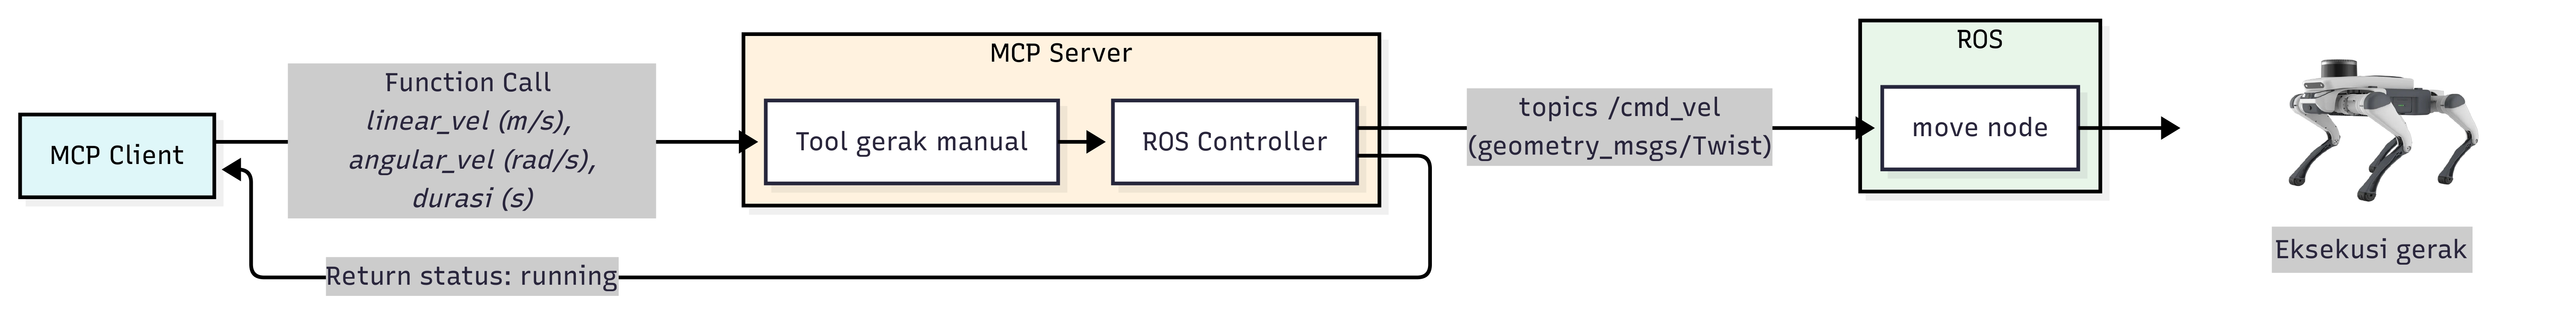
\includegraphics[width=1.0\textwidth]{Init/diagram-mcp-server/tool_gerak_manual.jpg}
    \caption{Diagram \textit{Tool} Gerak Manual}
    \label{fig:diagram_tool_gerak_manual}
\footnotesize \textbf{Sumber:} Dokumentasi Penulis
\end{figure}
Seperti yang diilustrasikan pada Gambar \ref{fig:diagram_tool_gerak_manual}, \textit{tool} gerak manual berfungsi untuk menggerakkan robot secara langsung tanpa menggunakan koordinat. \textit{Tool} ini menerima parameter masukan berupa kecepatan linear dalam satuan meter per detik (m/s), kecepatan angular dalam satuan radian per detik (rad/s), serta durasi pergerakan dalam satuan detik (s). Di dalam implementasinya, server akan memanggil \textit{ROS Controller} untuk mempublikasikan nilai kecepatan tersebut ke topik robot selama durasi waktu yang ditentukan. Proses ini berjalan secara asinkron sehingga server langsung mengembalikan status pengerjaan berupa running kepada client untuk menandakan perintah sedang dikirimkan, sehingga client tidak terblokir selama robot bergerak.

\subsubsection{\textit{Tool} Navigasi}
\begin{figure}[H]
    \centering
    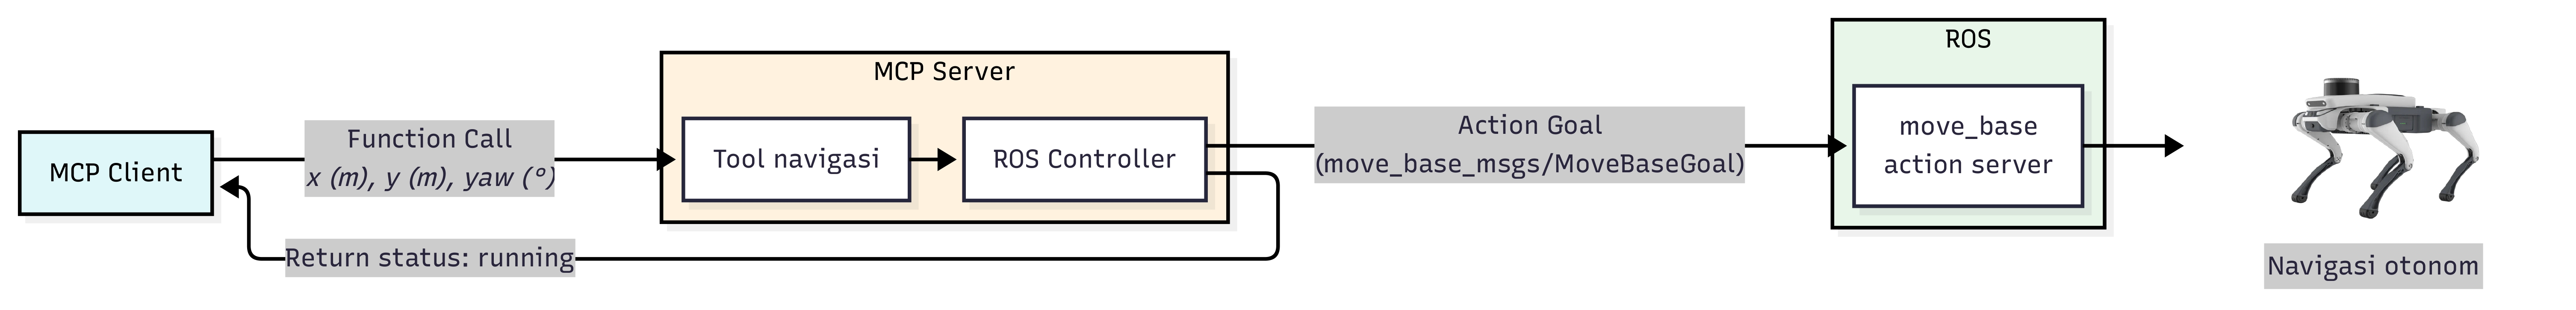
\includegraphics[width=1.0\textwidth]{Init/diagram-mcp-server/tool_navigasi.jpg}
    \caption{Diagram \textit{Tool} Navigasi}
    \label{fig:diagram_tool_navigasi}
\footnotesize \textbf{Sumber:} Dokumentasi Penulis
\end{figure}
Seperti yang ditunjukkan pada Gambar \ref{fig:diagram_tool_navigasi}, \textit{tool} navigasi digunakan untuk mengarahkan robot menuju suatu titik koordinat tujuan yang telah ditentukan pada peta. Parameter masukan untuk \textit{tool} ini meliputi koordinat X dan Y dalam satuan meter (m) pada kerangka acuan peta, serta sudut orientasi atau \textit{yaw} dalam satuan derajat ($^\circ$). Di dalam server, sudut orientasi dalam derajat terlebih dahulu dikonversi ke satuan radian (rad). Setelah itu, server mengirimkan koordinat tujuan tersebut ke server aksi navigasi move base yang ada pada ROS. Jika pengiriman koordinat tujuan berhasil dilakukan, server akan mengembalikan respons status running yang menandakan bahwa robot sedang dalam perjalanan menuju lokasi tujuan.

\subsubsection{\textit{Tool Toggle Sit/Stand} }
\begin{figure}[H]
    \centering
    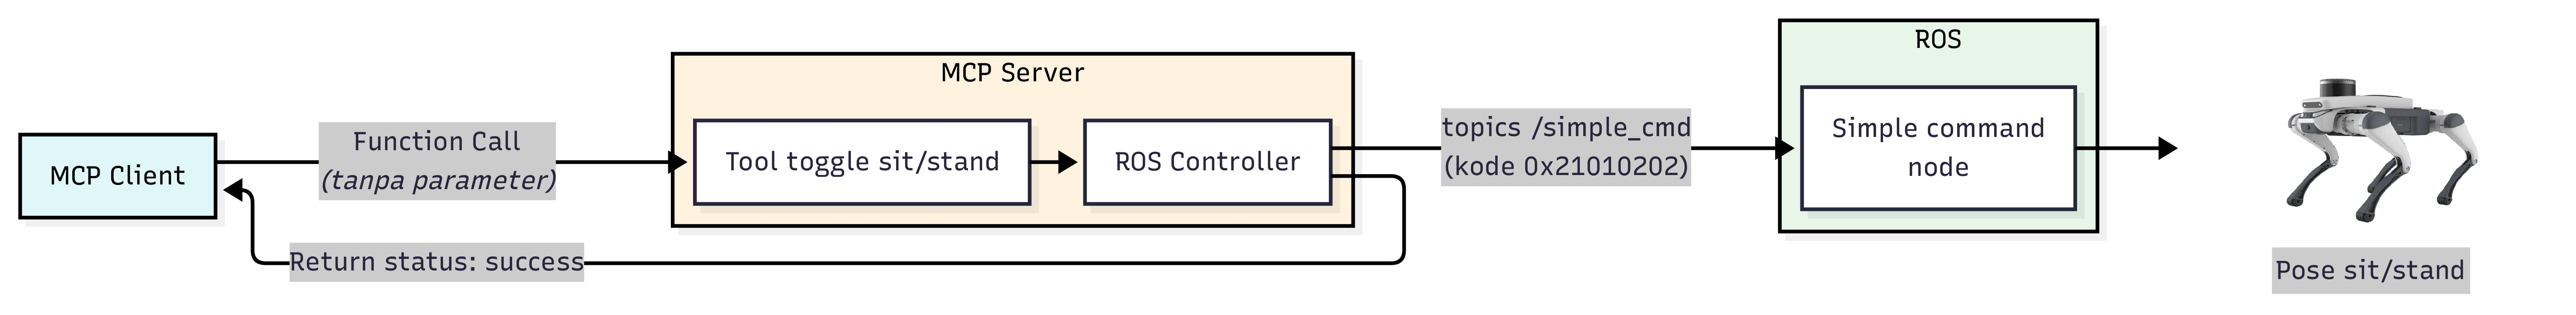
\includegraphics[width=1.0\textwidth]{Init/diagram-mcp-server/tool_toggle_sit_stand.jpg}
    \caption{Diagram \textit{Tool Toggle Sit/Stand}}
    \label{fig:diagram_tool_sitstand}
\footnotesize \textbf{Sumber:} Dokumentasi Penulis
\end{figure}
Seperti yang divisualisasikan pada Gambar \ref{fig:diagram_tool_sitstand}, \textit{tool} kontrol pose tubuh digunakan untuk mengubah pose berdiri atau duduk pada robot quadruped. \textit{Tool} ini tidak membutuhkan parameter masukan tambahan dari operator. Saat dijalankan, server akan memanggil fungsi pada \textit{ROS Controller} untuk mengirimkan perintah biner khusus dengan kode 0x21010202 ke sistem motor robot. Perintah tersebut memicu transisi fisik robot dari posisi berdiri ke posisi duduk atau sebaliknya. Setelah kode perintah sukses dikirimkan ke perangkat keras robot, \textit{tool} ini akan mengembalikan status sukses kepada client.

\subsubsection{\textit{Tool} Kontrol \textit{Pitch} Robot}
\begin{figure}[H]
    \centering
    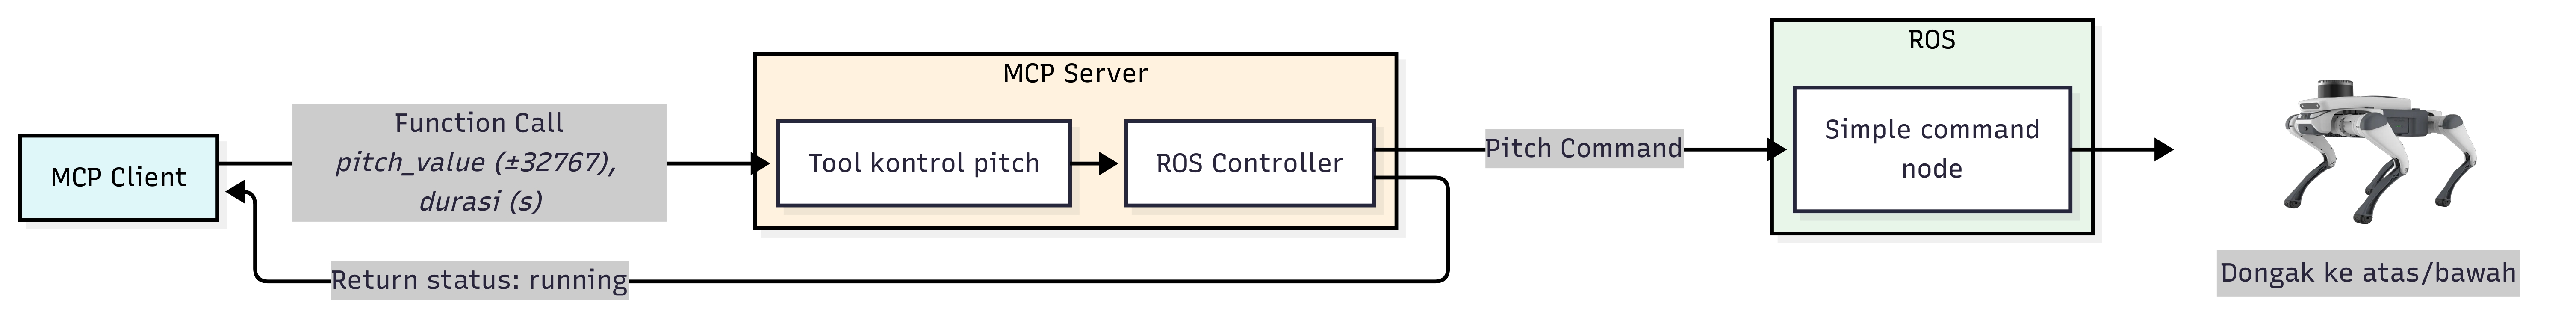
\includegraphics[width=1.0\textwidth]{Init/diagram-mcp-server/tool_pitch.jpg}
    \caption{Diagram \textit{Tool} Kontrol \textit{Pitch} Robot}
    \label{fig:diagram_tool_pitch}
\footnotesize \textbf{Sumber:} Dokumentasi Penulis
\end{figure}
Seperti yang diilustrasikan pada Gambar \ref{fig:diagram_tool_pitch}, \textit{tool} kontrol \textit{pitch} robot berfungsi untuk mengubah sudut kemiringan \textit{pitch} tubuh robot agar kamera dapat mendongak ke atas atau menunduk ke bawah secara dinamis. \textit{Tool} ini menerima parameter masukan berupa nilai sudut kemiringan dengan rentang antara -32767 hingga 32767, serta durasi pose dalam satuan detik (s). Nilai masukan di antara -6553 dan 6553 didefinisikan sebagai zona mati sehingga akan diabaikan oleh sistem. Nilai positif digunakan untuk mengarahkan kamera ke bawah, sedangkan nilai negatif digunakan untuk mengarahkan kamera ke atas. Perintah ini diproses secara asinkron oleh \textit{ROS Controller} untuk mengatur motor sendi robot selama durasi waktu yang diinginkan sebelum postur tubuh kembali ke kondisi normal.

\subsubsection{\textit{Tool} Pencarian Koordinat \textit{Waypoint}}
\begin{figure}[H]
    \centering
    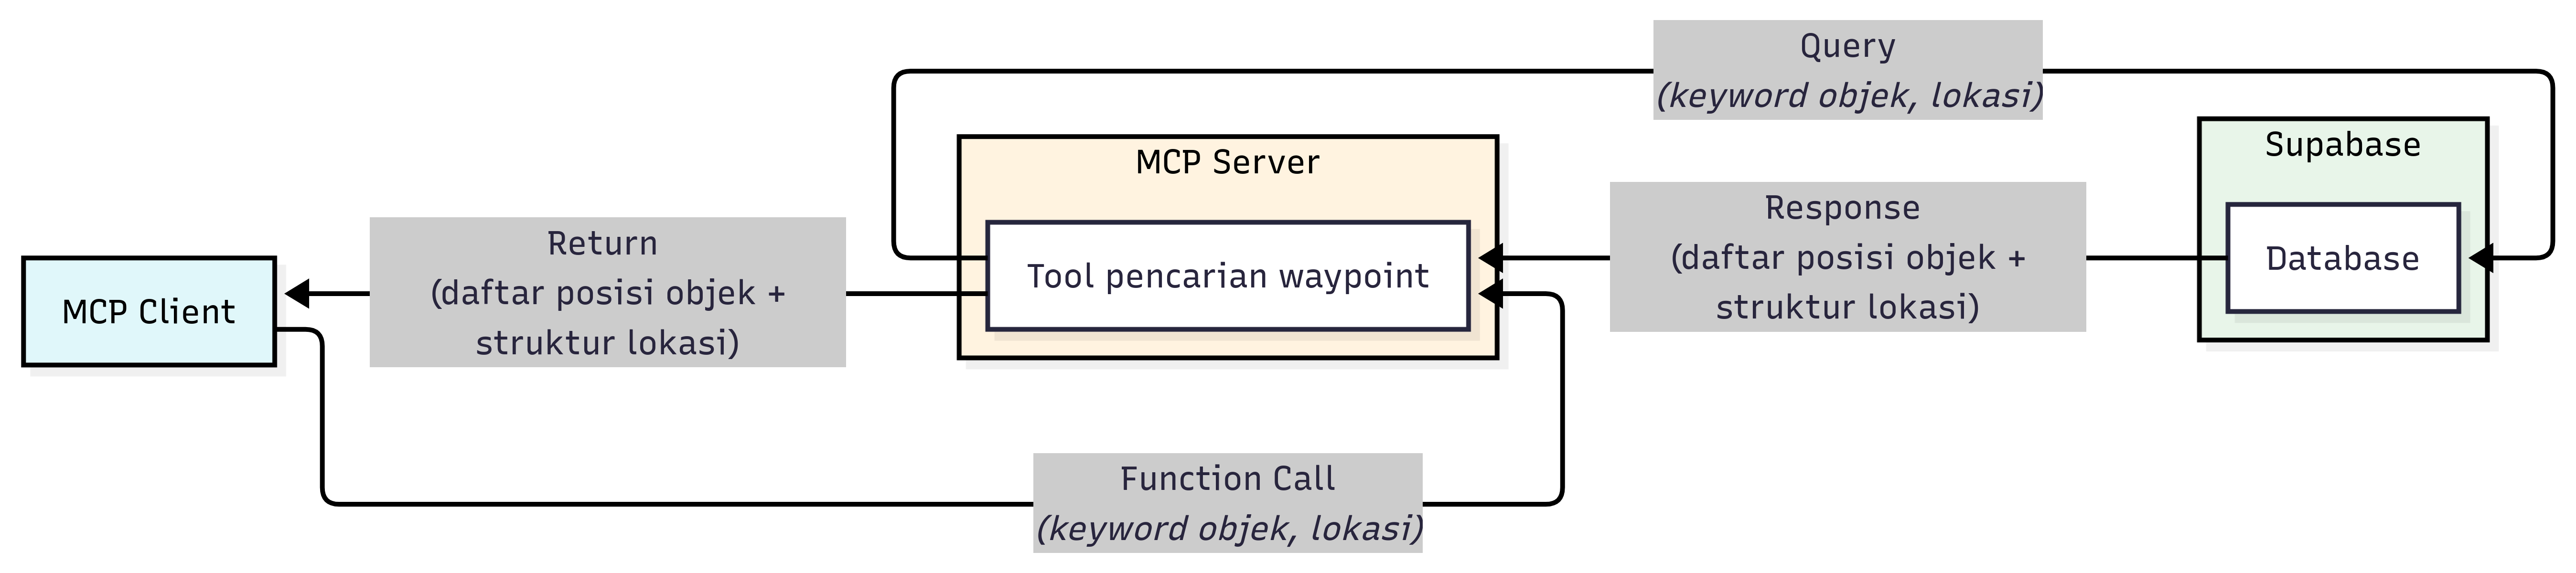
\includegraphics[width=1.0\textwidth]{Init/diagram-mcp-server/tool_waypoint.png}
    \caption{Diagram \textit{Tool} Pencarian Koordinat \textit{Waypoint}}
    \label{fig:diagram_tool_waypoint}
\footnotesize \textbf{Sumber:} Dokumentasi Penulis
\end{figure}
Seperti yang ditunjukkan pada Gambar \ref{fig:diagram_tool_waypoint}, \textit{tool} pencarian koordinat waypoint berfungsi untuk mencari lokasi fisik dan koordinat tujuan navigasi dari objek inspeksi yang terdaftar di dalam basis data. \textit{Tool} ini menerima parameter masukan berupa kata kunci nama objek serta parameter opsional berupa nama lokasi pencarian. Di dalam server, kueri dilakukan ke beberapa tabel basis data Supabase meliputi tabel objek, tabel waypoint, tabel lokasi, dan tabel peta. Server kemudian menyusun struktur lokasi secara hierarkis dari level peta hingga objek spesifik, serta mengekstrak data koordinat navigasi posisi target objek. Informasi tersebut dikirimkan dalam format data terstruktur kepada client.

\subsubsection{\textit{Tool} Pencarian Berkas SOP}
\begin{figure}[H]
    \centering
    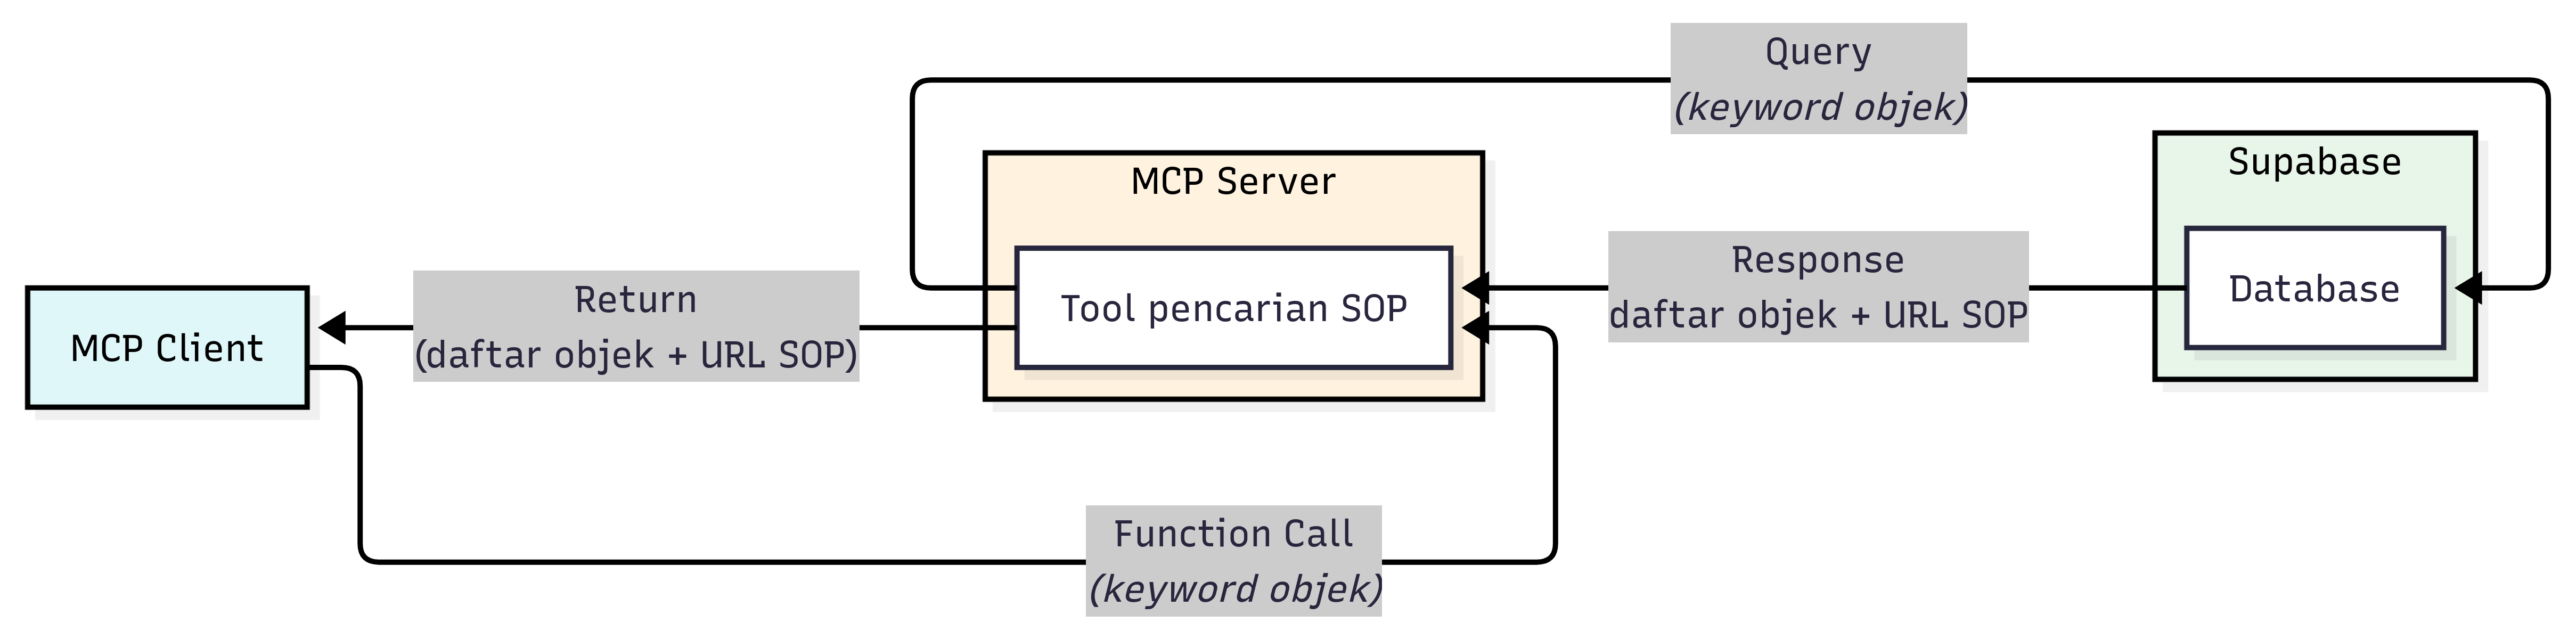
\includegraphics[width=1.0\textwidth]{Init/diagram-mcp-server/tool_sop.png}
    \caption{Diagram \textit{Tool} Pencarian Berkas SOP}
    \label{fig:diagram_tool_sop}
\footnotesize \textbf{Sumber:} Dokumentasi Penulis
\end{figure}
Seperti yang divisualisasikan pada Gambar \ref{fig:diagram_tool_sop}, \textit{tool} ini bertujuan untuk mencari  dokumen \textit{Standard Operating Procedure} (SOP) di dalam basis data. Agen AI cukup mengirimkan parameter masukan berupa nama objek atau kata kunci, lalu \textit{tool} ini akan melakukan pencarian kueri ke basis data dan mengembalikan daftar objek beserta tautan (\textit{URL}) berkas SOP yang berelasi dengannya. \textit{Tool} ini secara spesifik dirancang untuk hanya memberikan meta-informasi tanpa langsung mengekstrak isi teks dokumen guna menghemat penggunaan token pada jendela konteks model bahasa. Proses pengunduhan dokumen dari \textit{cloud storage} serta ekstraksi teks secara mendalam (baik dari format PDF maupun DOCX) akan dijalankan secara otomatis oleh MCP client di belakang layar.

\subsubsection{\textit{Tool} Pengambilan dan Analisis \textit{Image}}
\begin{figure}[H]
    \centering
    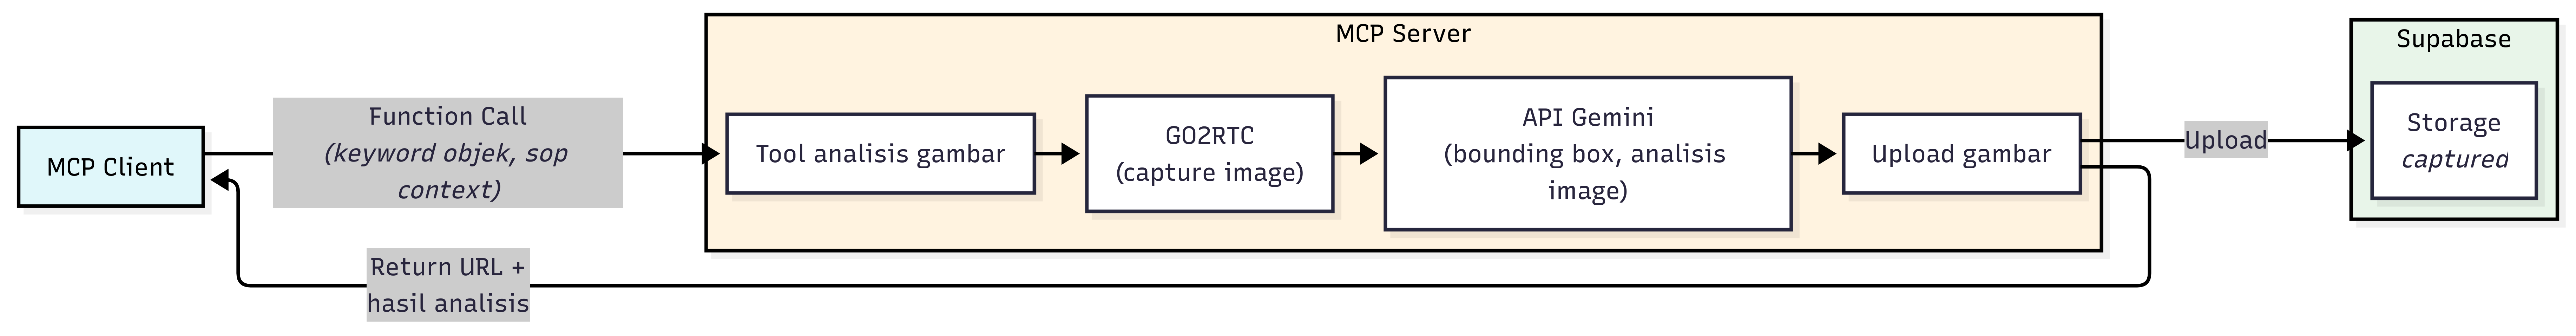
\includegraphics[width=1.0\textwidth]{Init/diagram-mcp-server/tool_analisis_image.png}
    \caption{Diagram \textit{Tool} Pengambilan dan Analisis \textit{Image}}
    \label{fig:diagram_tool_analisis}
\footnotesize \textbf{Sumber:} Dokumentasi Penulis
\end{figure}
Seperti yang ditunjukkan pada Gambar \ref{fig:diagram_tool_analisis}, \textit{tool} pengambilan dan analisis \textit{image} inspeksi merupakan \textit{tool} utama untuk mendeteksi objek serta menganalisis kondisinya. \textit{Tool} ini menerima parameter berupa kata kunci objek yang diperiksa. Pertama, server mengambil \textit{image} mentah dari kamera robot melalui protokol snapshot go2rtc. Jika objek yang diperiksa didefinisikan, \textit{image} tersebut dikirim ke model Gemini beserta teks instruksi deteksi objek. Model Gemini akan mengembalikan koordinat pembatas objek dalam bentuk bilangan bulat ternormalisasi. \textit{Image} mentah kemudian dipotong menggunakan modul OpenCV berdasarkan koordinat tersebut dengan menambahkan \textit{margin} sebesar 20 persen (\%) agar objek fokus di tengah. Jika teks prosedur standar disertakan, model Gemini akan menganalisis visual objek dan mengembalikan temuan inspeksi, analisis rinci, serta status kelayakan objek berupa normal, abnormal, atau tidak meyakinkan. \textit{Image} hasil pemrosesan kemudian diunggah ke penyimpanan Supabase dan server mengembalikan tautan publik beserta data analisis terstruktur kepada client.

\subsection{Sistem ROS}
Sistem perangkat lunak robot quadruped ini berjalan di atas Robot Operating System atau ROS dengan memanfaatkan repositori bawaan DeepRobotics yang dimodifikasi. Sistem ROS tersebut bertanggung jawab atas koordinasi sensor, navigasi, lokalisasi, pemetaan lingkungan sekitar, serta penerjemahan data telemetri.

\subsubsection{Lokalisasi dan Pemetaan SLAM} 
\begin{figure}[h!]
    \centering
    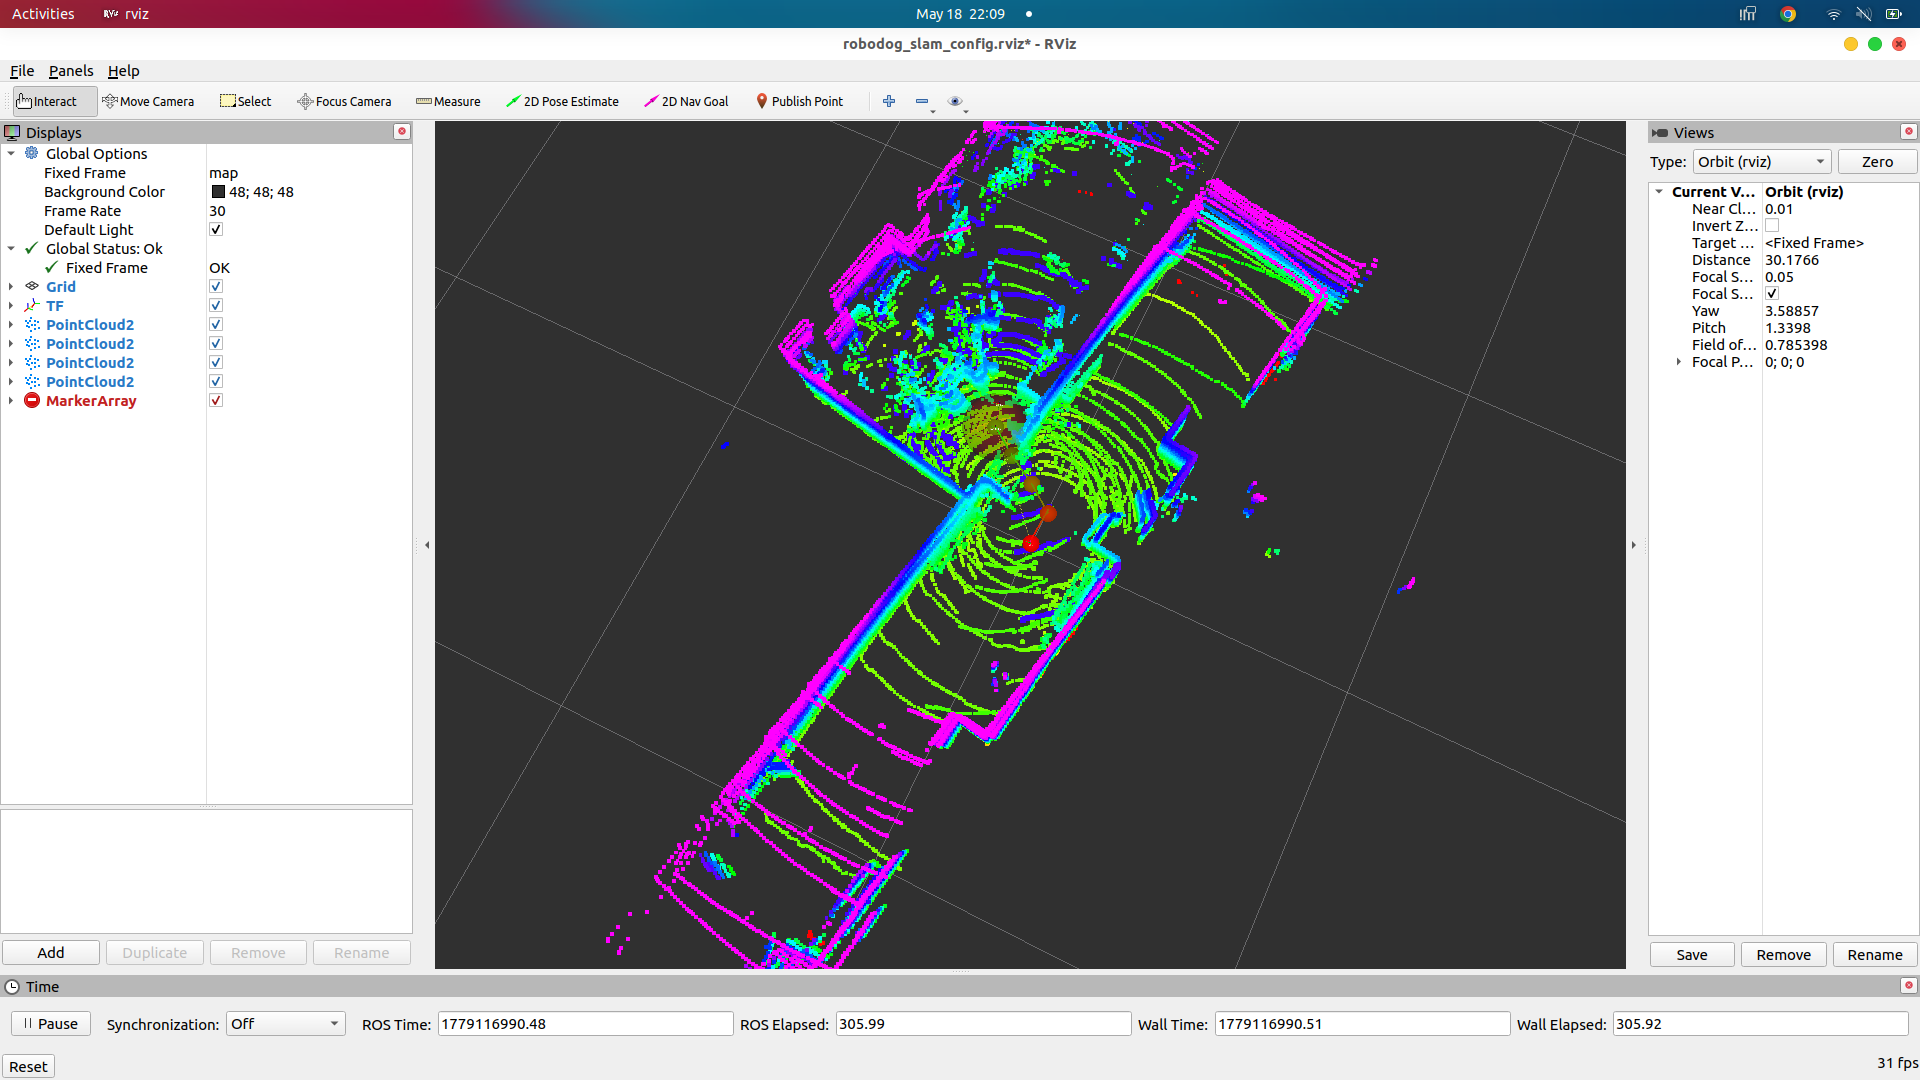
\includegraphics[width=1.0\textwidth]{Init/gambar/mapping.png}
    \caption{Proses pemetaan dan lokalisasi pada Robot}
    \label{fig:mapping}
\footnotesize \textbf{Sumber:} Dokumentasi Penulis
\end{figure}
Sebagaimana diilustrasikan pada diagram Gambar \ref{fig:mapping}, proses lokalisasi dan pemetaan lingkungan dilakukan dengan memanfaatkan algoritma pemetaan yang sudah tersedia pada sistem bawaan robot. Proses ini dijalankan dengan mengeksekusi \textit{executable file} pemetaan dari repositori bawaan yang secara otomatis bertugas menerima dan memproses data pindaian \textit{point cloud} tiga dimensi dari sensor LiDAR. Sistem pemetaan bawaan ini digunakan secara praktis tanpa melakukan perancangan algoritma pemetaan baru ataupun modifikasi pemrosesan tingkat rendah. Hasil akhir dari proses pemetaan ini berupa peta \textit{point cloud} tiga dimensi yang kemudian disimpan dan digunakan sebagai peta acuan utama navigasi bagi robot.

\subsubsection{Navigasi} 
\begin{figure}[H]
    \centering
    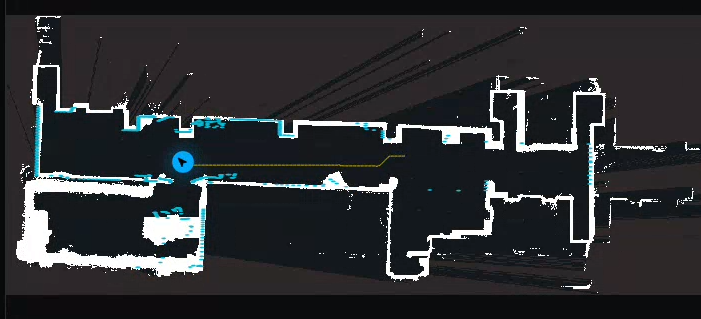
\includegraphics[width=1.0\textwidth]{Init/gambar/navigasi.png}
    \caption{Proses navigasi pada Robot}
    \label{fig:navigasi}
\footnotesize \textbf{Sumber:} Dokumentasi Penulis
\end{figure}
Proses navigasi otonom robot diaktifkan melalui antarmuka web operator dengan menekan tombol inisialisasi. Aksi ini akan memicu skrip inisialisasi navigasi pada komputer robot yang bertugas memuat peta lingkungan yang telah dibuat sebelumnya. Skrip ini meluncurkan komponen pencarian posisi lokal berbasis pencocokan pindaian LiDAR tiga dimensi yang dikombinasikan dengan data dari sensor inersia atau IMU. Hal tersebut memungkinkan robot mengetahui lokasinya secara presisi dalam koordinat peta tanpa harus bergantung pada sensor eksternal. Sistem navigasi ini menggunakan \textit{navigation stack} yang mengintegrasikan perencana jalur global untuk mencari rute terpendek dan perencana jalur lokal untuk menghindari rintangan dinamis secara real-time. Sebuah contoh dari proses navigasi robot menuju satu titik tujuan dapat dilihat pada Gambar \ref{fig:navigasi}.

\subsubsection{\textit{RosBridge WebSocket}}
\begin{figure}[H]
    \centering
    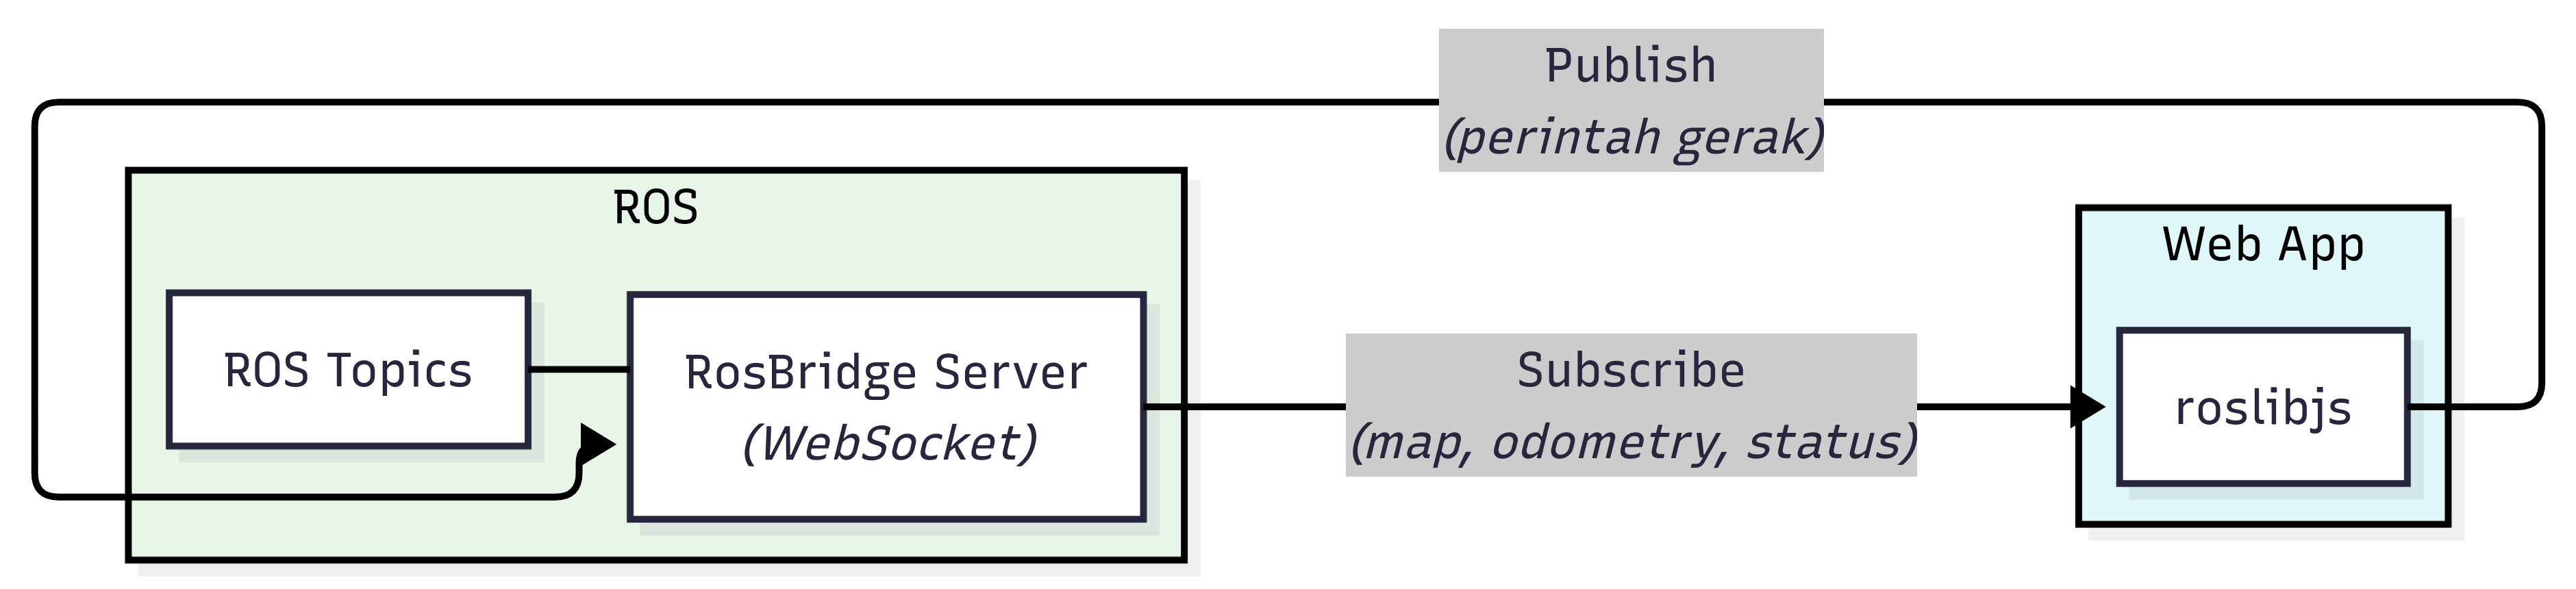
\includegraphics[width=0.8\textwidth]{Init/diagram-ros/rosbridge.png}
    \caption{Diagram \textit{RosBridge WebSocket}}
    \label{fig:diagram_rosbridge}
\footnotesize \textbf{Sumber:} Dokumentasi Penulis
\end{figure}
Seperti yang diilustrasikan pada Gambar \ref{fig:diagram_rosbridge}, komunikasi dua arah antara aplikasi antarmuka web dengan sistem ROS di dalam robot difasilitasi oleh modul \textit{rosbridge suite}. Modul ini menjalankan server WebSocket pada port 9090 di dalam komputer robot. Antarmuka web menggunakan pustaka \textit{roslibjs} untuk melakukan koneksi ke WebSocket tersebut, sehingga operator dapat mengirimkan perintah gerak, menerima data status robot, menerima data peta, serta data koordinat secara langsung. Penggunaan protokol ini sangat efisien karena data dipertukarkan dalam format teks JSON secara asinkron.

\subsubsection{ROS \textit{Messages Transformer}}
\begin{figure}[H]
    \centering
    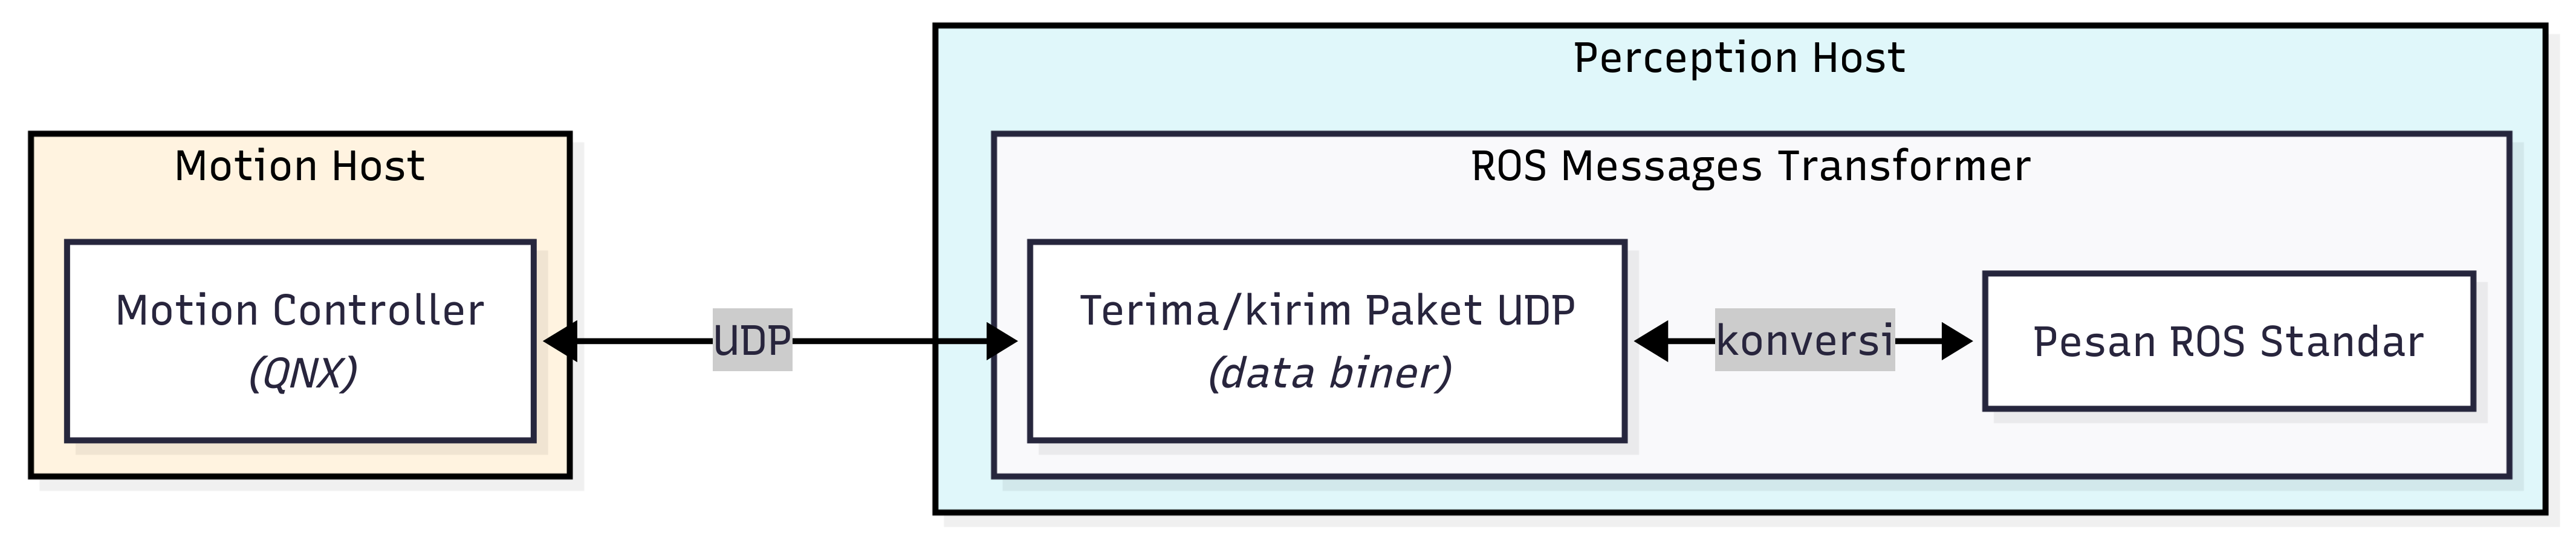
\includegraphics[width=0.8\textwidth]{Init/diagram-ros/msg_transformer.png}
    \caption{Diagram ROS \textit{Messages Transformer}}
    \label{fig:diagram_msg_transformer}
\footnotesize \textbf{Sumber:} Dokumentasi Penulis
\end{figure}
Seperti yang ditunjukkan pada Gambar \ref{fig:diagram_msg_transformer}, modul penerjemah pesan atau \textit{message transformer} digunakan untuk menjembatani komunikasi dua arah tingkat rendah antara sistem kendali gerak robot yang berjalan pada sistem operasi QNX di dalam \textit{Motion Host} dengan ekosistem ROS di \textit{Perception Host}. Pada arah masuk, modul ini menerima paket data biner melalui protokol UDP yang berisi parameter kecepatan motor, kondisi sendi, serta data sensor inersia dari \textit{Motion Controller}, kemudian mengemasnya kembali menjadi pesan ROS standar. Pada arah keluar, modul ini juga menerjemahkan perintah pergerakan dari topik ROS menjadi paket data biner UDP yang dikirimkan ke \textit{Motion Controller} untuk menggerakkan aktuator fisik robot. Untuk memenuhi kebutuhan pemantauan \textit{real-time} pada antarmuka web, modul ini dimodifikasi dengan menambahkan fungsionalitas ekstra berupa ekstraksi informasi kapasitas baterai dan status dasar robot. Data tersebut kemudian dipublikasikan ke dalam topik ROS /battery\_level dan /robot\_basic\_state yang memungkinkan data tersebut disalurkan melalui rosbridge ke aplikasi antarmuka pengguna.

\subsection{Implementasi Basis Data}
\begin{figure}[h!]
    \centering
    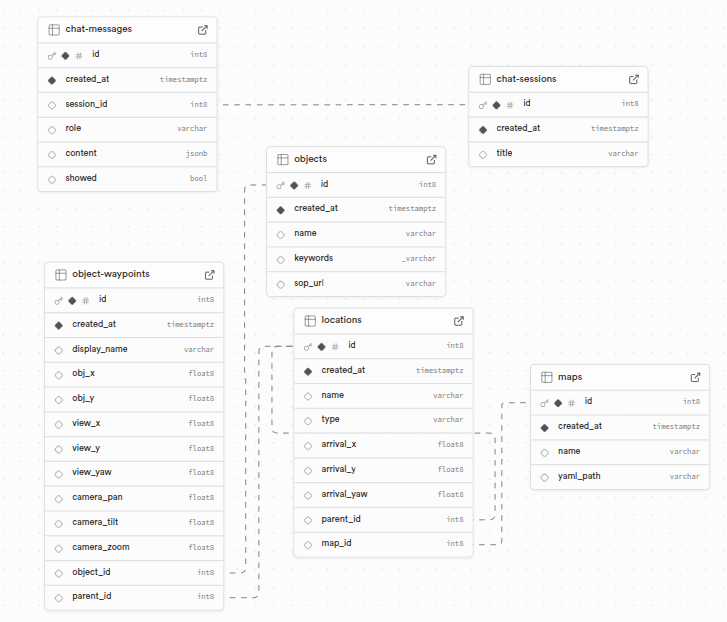
\includegraphics[width=1.0\textwidth]{Init/gambar/database.png}
    \caption{ERD Supabase}
    \label{fig:ERD}
\footnotesize \textbf{Sumber:} Dokumentasi Penulis
\end{figure}
Sistem ini menggunakan Supabase sebagai penyedia layanan basis data relasional berbasis PostgreSQL. Basis data ini dirancang untuk menyimpan data spasial lingkungan kerja robot, informasi koordinat objek inspeksi, berkas prosedur operasi standar, serta seluruh riwayat percakapan antara operator dan agen AI. Hubungan antartabel di dalam basis data dirancang secara relasional untuk menjamin konsistensi data koordinat serta memudahkan proses kueri yang dilakukan oleh server. Hubungan relasional antartabel basis data ini dapat dilihat pada Gambar \ref{fig:ERD}.

\subsubsection{Tabel \textit{Maps}}
Tabel maps berfungsi untuk menyimpan metadata peta lingkungan dua dimensi maupun tiga dimensi yang telah dihasilkan oleh robot. Tabel ini memiliki kolom id sebagai \textit{primary key} dengan tipe data bilangan bulat yang bersifat inkremental. Kolom created\_at mencatat waktu pembuatan data dengan tipe stempel waktu beserta zona waktu. Kolom name bertipe karakter digunakan untuk menyimpan nama peta yang mudah dipahami manusia. Kolom yaml\_path bertipe karakter menyimpan alamat jalur penyimpanan berkas konfigurasi peta pada sistem robot. Tabel ini memiliki relasi \textit{one-to-many} dengan tabel lokasi. Di dalam sistem, data peta ini diakses oleh aplikasi antarmuka web Next.js saat operator memilih profil peta awal sesi, serta digunakan oleh skrip inisialisasi navigasi untuk memuat berkas konfigurasi peta acuan.

\subsubsection{Tabel \textit{Locations}}
Tabel locations dirancang untuk memodelkan struktur hierarki lokasi fisik di dalam area kerja robot, seperti gedung, lantai, atau ruangan tertentu. Tabel ini memiliki kolom id sebagai \textit{primary key}. Kolom created\_at mencatat waktu pembuatan data. Kolom name menyimpan nama lokasi dan kolom type menentukan kategori lokasi seperti ruangan atau lantai. Kolom arrival\_x, arrival\_y, dan arrival\_yaw bertipe angka desimal digunakan untuk menyimpan koordinat tujuan kedatangan robot saat memasuki lokasi tersebut. Kolom parent\_id merupakan \textit{foreign key} yang merujuk kembali ke kolom \textit{primary key} tabel ini sendiri untuk membentuk hubungan hierarkis bertingkat. Kolom map\_id merupakan \textit{foreign key} yang merujuk ke tabel peta untuk mengaitkan lokasi dengan peta acuan yang digunakan. Tabel ini digunakan oleh halaman navigasi spasial pada antarmuka web untuk menampilkan struktur lokasi, serta dibaca oleh MCP server untuk mendapatkan peta semantik.

\subsubsection{Tabel \textit{Objects}}
Tabel objects menyimpan daftar tipe objek fisik yang menjadi target inspeksi oleh robot. Tabel ini memiliki kolom id sebagai \textit{primary key} dan kolom created\_at untuk stempel waktu. Kolom name digunakan untuk menyimpan nama jenis objek inspeksi. Kolom keywords bertipe \textit{array} teks digunakan oleh agen AI untuk mencocokkan nama objek yang ditanyakan oleh operator. Kolom sop\_url bertipe karakter menyimpan tautan menuju berkas prosedur standar inspeksi objek tersebut. Tabel ini dibaca oleh \textit{tool} pencari koordinat objek pada MCP Server saat melakukan pencocokan kata kunci objek yang dikirim oleh agen AI.

\subsubsection{Tabel \textit{Object Waypoints}}
Tabel object-waypoints berfungsi untuk menghubungkan objek inspeksi dengan koordinat objek. Tabel ini memiliki kolom id sebagai \textit{primary key} dan kolom created\_at untuk stempel waktu. Kolom display\_name menyimpan nama titik inspeksi. Kolom obj\_x dan obj\_y menyimpan estimasi koordinat lokasi objek itu sendiri. Kolom view\_x, view\_y, dan view\_yaw menyimpan koordinat navigasi yang harus dicapai robot untuk dapat melihat objek dengan baik. Kolom camera\_pan, camera\_tilt, dan camera\_zoom menyimpan parameter konfigurasi sudut kamera agar mengarah tepat ke objek. Kolom object\_id bertipe \textit{foreign key} yang merujuk ke tabel objek, sedangkan kolom parent\_id bertipe \textit{foreign key} yang merujuk ke tabel lokasi. Data dari tabel ini digunakan oleh \textit{tool} pencari koordinat objek pada MCP Server untuk mendapatkan target koordinat navigasi yang dikirimkan ke stack navigasi ROS.

\subsubsection{Tabel \textit{Chat Sessions}}
Tabel chat-sessions digunakan untuk mencatat setiap sesi percakapan baru yang diinisialisasi oleh operator melalui antarmuka pengguna. Tabel ini memiliki kolom id sebagai \textit{primary key}. Kolom created\_at mencatat stempel waktu inisialisasi sesi. Kolom title bertipe karakter digunakan untuk menyimpan judul sesi percakapan guna memudahkan pencarian riwayat oleh operator. Tabel ini memiliki relasi \textit{one-to-many} dengan tabel pesan percakapan. Tabel ini diakses oleh MCP client untuk membuat sesi baru dan menampilkan daftar sesi percakapan yang telah ada pada antarmuka web.

\subsubsection{Tabel \textit{Chat Messages}}
Tabel chat-messages berfungsi untuk menyimpan seluruh riwayat pesan di dalam setiap sesi percakapan secara terperinci. Tabel ini memiliki kolom id sebagai \textit{primary key} dan kolom created\_at sebagai stempel waktu pengiriman pesan. Kolom session\_id bertipe \textit{foreign key} yang merujuk ke tabel sesi percakapan untuk mengelompokkan pesan. Kolom role bertipe karakter menentukan pengirim pesan, seperti pengguna, asisten model, atau sistem \textit{tool}. Kolom content bertipe format data JSON digunakan untuk menyimpan teks percakapan. Kolom showed bertipe boolean dengan nilai bawaan benar digunakan untuk mengontrol apakah pesan tersebut harus ditampilkan di halaman antarmuka pengguna atau hanya dibaca sebagai riwayat konteks oleh agen AI. Tabel ini terhubung erat dengan antarmuka percakapan web yang menampilkan pesan secara dinamis. Modul MCP client menulis pesan baru ke tabel ini, dan perubahan data langsung memicu pembaruan pada tampilan antarmuka web secara real-time. Web juga membaca tabel ini untuk menampilkan percakapan saat ini dan memuat riwayat percakapan lama ketika operator memilih sesi tertentu.

\subsubsection{Supabase \textit{Storage}}
Selain tabel relasional, sistem ini menggunakan Supabase Storage sebagai wadah penyimpanan berkas objek tidak terstruktur. Penyimpanan ini dibagi menjadi dua folder utama. Folder pertama yaitu folder prosedur standar yang bertugas menyimpan dokumen panduan inspeksi objek dalam format dokumen. Folder ini dibaca oleh \textit{tool} pencari dokumen prosedur pada MCP Server untuk mengunduh dokumen panduan inspeksi. Folder kedua yaitu folder \textit{image} hasil tangkapan yang berfungsi untuk menyimpan foto mentah dari kamera robot serta foto hasil pemotongan fokus objek inspeksi. Setiap berkas yang diunggah ke dalam folder \textit{image} akan menghasilkan alamat tautan publik yang nantinya disimpan pada kolom konten di tabel pesan percakapan agar dapat ditampilkan langsung ke layar operator. Folder ini diakses oleh \textit{tool} pengambilan \textit{image} pada MCP Server untuk menyimpan \textit{image}. Storage ini juga digunakan oleh MCP Client untuk mengunduh berkas dokumen SOP dan \textit{image} hasil inspeksi agar dapat disisipkan kembali ke dalam konteks percakapan model bahasa Gemini. Web juga membaca storage ini untuk menampilkan \textit{image} dan dokumen SOP pada halaman terkait.